%%%%%%%%%%%%%%%%%%%%%%%[Comments]%%%%%%%%%%%%%%%%%%%%%%%

% ******* If you want the true bare-bone structure, go to ********
% https://github.com/taehoonlee/snu-dissertation-template

%%%%%%%%%%%%%%%%%%%%%%%%%%%%%%%%%%%%%%%%%%%%%%%%%%%%%%%%

\documentclass[12pt]{report}
\usepackage[paperwidth=21cm,paperheight=29.7cm,left=2.5cm,right=2.5cm,top=3.5cm,bottom=1.5cm]{geometry}
% Originally this was
%\usepackage[paperwidth=19cm,paperheight=26cm,left=3cm,right=3cm,top=3.5cm,bottom=1.5cm]{geometry}

\addtolength{\voffset}{-1.5cm}
\renewcommand{\baselinestretch}{1.7}
\renewcommand{\abstractname}{\large Abstract}
\usepackage{setspace}
\usepackage[]{enumitem}
%\usepackage{lmodern}
%\usepackage{librecaslon}
\usepackage[T1]{fontenc}
\usepackage{footnote}
\usepackage{textcomp}
\usepackage{kotex}
\usepackage{tabularx}
\usepackage{makecell}
\usepackage{graphicx}
\usepackage{multirow}

\newtheorem{definition}{Definition}[section]
\newtheorem{example}{Example}[section]
\newtheorem{theorem}{Theorem}[section]
\newtheorem{lemma}{Lemma}[section]
\newtheorem{corollary}{Corollary}[section]
\newtheorem{pf}{Proof}[section]
%%%%%%%%%%%%%%%%%%%%%%%%%%%%%%%%%%%%%%%%
% Reference style settings
% ↓ This is also free to change. Do as you wish...
\usepackage[numbers,square]{natbib}


%%%%%%%%%%%%%%%%%%%%
% Page numbering style settings
% For proper page numbering at TOC part https://tex.stackexchange.com/questions/235866/page-number-resets-on-table-of-contents
\makeatletter
\renewenvironment{abstract}{%
    \if@twocolumn
    \section*{\abstractname}%
    \else
    \small
    \begin{center}%
        {\bfseries \abstractname\vspace{-.5em}\vspace{\z@}}%
    \end{center}%
    \quotation
    \fi}
{\if@twocolumn\else\endquotation\fi}
\makeatother
%%%%%%%%%%%%%%%%%%%%

%↓↓↓↓↓↓↓↓↓↓[Free to change, preamble. START]↓↓↓↓↓↓↓↓↓↓
% It is your choice to change contents from here to the end of preamble.

\usepackage{amsmath,amssymb}
\usepackage{tikz}
\usepackage{mathtools}
\usepackage{graphicx}
\usepackage{siunitx}
\usepackage{physics}
\usepackage{rotating}  % The package to rotate table by sidewaystable
\usepackage{csquotes}  % for ``displayquote`` environment
\usepackage[notextcomp]{stix}  % without notextcomp, "Option clash for package textcomp." error pops up...
%\usepackage[libertine,cmintegrals,cmbraces,vvarbb]{newtxmath}
\usepackage[font=small]{caption}
\usepackage{listings}
\usepackage{xcolor}


%%%%%%%%%%%%%%%%%%%%
% For URL-ed A&A style bibliography (https://github.com/yangcht/AA-bibstyle-with-hyperlink)
% IMPORTANT NOTE:
% As of 2023-05-18, at least PHDTHESIS must have `adsurl={}` and `adsnote={}`, when they are not registered to ADS. If they don't have these fields, """Extra }, or forgotten \endgroup. """ error will appear.
\usepackage{twoopt}
\usepackage[breaklinks]{hyperref}      %% to avoid \citeads line fills, add "draft"
                                       %% to avoid the PDFTK error (broken links)
% \bibpunct{(}{)}{;}{a}{}{,}             %% natbib format for A&A and ApJ
\definecolor{cobalt}{rgb}{0.06, 0.2, 0.65}
\hypersetup{
  colorlinks,
  citecolor=cobalt,
  linkcolor=[rgb]{0.8, 0.2, 1.0},
  urlcolor=cobalt,
}
% \makeatletter
%   \newcommandtwoopt{\citeads}[3][][]{\href{http://adsabs.harvard.edu/abs/#3}%
%     {\def\hyper@linkstart##1##2{}%
%      \let\hyper@linkend\@empty\citealp[#1][#2]{#3}}}
%   \newcommandtwoopt{\citepads}[3][][]{\href{http://adsabs.harvard.edu/abs/#3}%
%     {\def\hyper@linkstart##1##2{}%
%      \let\hyper@linkend\@empty\citep[#1][#2]{#3}}}
%   \newcommandtwoopt{\citetads}[3][][]{\href{http://adsabs.harvard.edu/abs/#3}%
%     {\def\hyper@linkstart##1##2{}%
%      \let\hyper@linkend\@empty\citet[#1][#2]{#3}}}
%   \newcommandtwoopt{\citeyearads}[3][][]%
%     {\href{http://adsabs.harvard.edu/abs/#3}
%     {\def\hyper@linkstart##1##2{}%
%      \let\hyper@linkend\@empty\citeyear[#1][#2]{#3}}}
% \makeatother
%%%%%%%%%%%%%%%%%%%%

\usepackage{url}
%\usepackage{hyperref}
\usepackage{cleveref}

%\crefname{equation}{equation}{equations}%
%\crefname{chapter}{chapter}{chapters}%
%\crefname{section}{section}{sections}%
%\crefname{appendix}{appendix}{appendices}%
%\crefname{enumi}{item}{items}%
%\crefname{footnote}{footnote}{footnotes}%
%\crefname{figure}{figure}{figures}%
%\crefname{table}{table}{tables}%
%\crefname{theorem}{theorem}{theorems}%
%\crefname{lemma}{lemma}{lemmas}%
%\crefname{corollary}{corollary}{corollaries}%
%\crefname{proposition}{proposition}{propositions}%
%\crefname{definition}{definition}{definitions}%
%\crefname{result}{result}{results}%
%\crefname{example}{example}{examples}%
%\crefname{remark}{remark}{remarks}%
%\crefname{note}{note}{notes}%

\Crefname{equation}{Eq.}{Eqs.}%
\Crefname{chapter}{Chap.}{Chaps.}%
\Crefname{section}{\S}{\S}%
\Crefname{appendix}{App.}{Apps.}%
\Crefname{enumi}{item}{items}%
\Crefname{footnote}{footnote}{footnotes}%
\Crefname{figure}{Fig.}{Figs.}%
\Crefname{table}{Tab.}{Tabs.}%
%\Crefname{theorem}{Thm.}{Thms.}%
%\Crefname{lemma}{Lem.}{Lems.}%
%\Crefname{corollary}{Cor.}{Cors.}%
%\Crefname{proposition}{proposition}{propositions}%
\Crefname{definition}{Def.}{Defs}%
%\Crefname{result}{result}{results}%
%\Crefname{example}{example}{examples}%
%\Crefname{remark}{remark}{remarks}%
%\lCrefname{note}{note}{notes}%

\makeatletter
\renewcommand*{\fps@figure}{tb}
\renewcommand*{\fps@table}{tb}
\makeatother

\renewenvironment{abstract}
 {\small
  \begin{center}
  \bfseries \abstractname\vspace{-.5em}\vspace{0pt}
  \end{center}
  \list{}{%
    \setlength{\leftmargin}{10mm}% <---------- CHANGE HERE
    \setlength{\rightmargin}{\leftmargin}%
  }%
  \item\relax}
 {\endlist}

%↑↑↑↑↑↑↑↑↑↑[Free to change, preamble. END]↑↑↑↑↑↑↑↑↑↑
%↑↑↑↑↑↑↑↑↑↑[여기까지 Setting(왜 필요한지는 모름)]↑↑↑↑↑↑↑↑↑↑

\begin{document}

\pagenumbering{gobble}

% ------------ Title ------------ %
\begin{titlepage}
% Thesis title
\def\tTitleA{{Deep Dive to Quantum Machine Learning}}
\def\tTitleB{{: focused on Imparting Non-Linearity}}
\def\tTitleK{{양자머신러닝의 수학적 원리와 확장}}
\def\tTitleKK{{: 비선형성 도입을 중심으로}}

% 후보 : Analysis of Quantum Machine Learning
% 후보 : 


% Department name
\def\tDepartment{{Department of Mathematics}}  % Department name
\def\tDepartmentKr{{학부 수학전공}}           % Department name
\def\tCollegeOrGradSchool{{College of Natural Sciences}}  % Exists only in English format.. I dunno why.
\def\tMajor{{Mathematics}}  % Normally it is in separate line in English version. If you have major, add this. Otherwise, modify below (cosmetically modify as you wish)

% Submission date.
% I have no idea about official regulation, but mostly people do 6월 or 12월.
\def\tDate{{June 2023}}
\def\tDateKr{{2023년 6월}}

% Only February or August
\def\tInjunDate{{December 2024}}
\def\tInjunDateKr{{2024년 12월}}  % xxxx년 2월 OR 8월

% Name of the degree
\def\tDeg{{Ph.D.}}
\def\tDegKr{{수학창의연구}}  % 이학석사, 이학박사, 공학석사, 공학박사, ...
\def\tDegLong{{Doctor of Philosophy}}

% My name
% \def\tName{{Gildong X. Hong}}
\def\tNameWithBlank{{한재훈 외 2인}}
% \def\tNameKr{{홍길동}}  % If you want, you can put English name here too (I did it with my PhD thesis)
% \def\tNameKrWithBlank{{홍\ 길\ 동}}  % If you want, you can put English name here too (I did it with my PhD thesis)

% Supervisor name
\def\tNameSuper{{Baksa\ F.\ Kim}}
\def\tNameSuperKr{{김\ 박\ 사}}   % If you want, you can put English name here too (I did it with my PhD thesis)


\newcommand{\wideunderline}[2][2em]{%
  \underline{\makebox[\ifdim\width>#1\width\else#1\fi]{#2}}%
}
%%%%%%%%%%%%%%%%%%%%%%%%%%%%%%%%%%%%%%%%%%
%% Korean Version
%%%%%%%%%%%%%%%%%%%%%%%%%%%%%%%%%%%%%%%%%%
\renewcommand{\baselinestretch}{1}
\centering
{\Large \quad \par}
\vspace{.5cm}{\Large \bf \tDegKr\ 결과보고서 \par}
\vspace{2cm}
{\Huge \bf \tTitleA \par}
\vspace{.3cm}
{\Huge \bf \tTitleB \par}
\vspace{2cm}
{\LARGE \bf \tTitleK \par}
\vspace{.3cm}
{\LARGE \bf \tTitleKK \par}
\vspace{4.5cm}
{\Large \bf \tInjunDateKr \par}
\vspace{3cm}
{\LARGE \bf 아주대학교 수학과 \par}  % I think it should be "서울대학교 대학원" all the time.
\vspace{.5cm}
{\Large \bf \tDepartmentKr \par}
\vspace{.5cm}
{\LARGE \bf \tNameWithBlank \par}



\clearpage

% \centering
% {\Large \quad \par}
% \vspace{.1cm}
% {\Huge \bf \tTitleA \par}
% \vspace{.3cm}
% {\Huge \bf \tTitleB \par}
% \vspace{0.5cm}
% {\LARGE \bf  \tTitleK \par}
% \vspace{1.cm}
% {\Large \bf 지도교수 $\ $ \tNameSuperKr  \par}
% \vspace{0.5cm}
% {\LARGE \bf 이 논문을 \tDegKr\ 학위논문으로 제출함 \par}
% \vspace{.2cm}
% {\Large \bf \tDateKr \par}

% \vspace{.9cm}
% {\LARGE \bf 서울대학교 대학원 \par}
% \vspace{.3cm}
% {\Large \bf \tDepartmentKr \par}
% \vspace{.3cm}
% {\LARGE \bf \tNameKrWithBlank \par}
% \vspace{.9cm}

% {\LARGE \bf \tNameKr 의 \tDegKr\ 학위논문을 인준함 \par}
% \vspace{.2cm}
% {\Large \bf \tInjunDateKr \par}
% \vspace{1.2cm}
% {\Large \bf  위\hspace{0.48cm}원\hspace{0.48cm}장} \quad {\Large \wideunderline[12em]{\hfill Professor N. One\hfill(인)}} \par
% \vspace{.7cm}
% {\Large \bf 부\ 위\ 원\ 장} \quad {\Large \wideunderline[12em]{\hfill Likely Ur. Supervisor\hfill(인)} } \par
% \vspace{.7cm}
% {\Large \bf 위\hspace{1.55cm}원} \quad {\Large \wideunderline[12em]{\hfill Another Professor\hfill(인)} } \par
% \vspace{.7cm}
% {\Large \bf  위\hspace{1.55cm}원} \quad {\Large \wideunderline[12em]{\hfill Another Doctor\hfill(인)} } \par
% \vspace{.7cm}
% {\Large \bf 위\hspace{1.55cm}원} \quad {\Large \wideunderline[12em]{\hfill Yet Another\hfill(인)} } \par


% %%%%%%%%%%%%%%%%%%%%%%%%%%%%%%%%%%%%%%%%%%
% %% An Information page in English
% %% I made it by myself following few predecessors. I don't know if this is an official format.
% %%%%%%%%%%%%%%%%%%%%%%%%%%%%%%%%%%%%%%%%%%
% \clearpage
% \centering

% {\Large \quad \par}
% \vspace{.1cm}
% {\Huge \bf \tTitleA \par}
% \vspace{.3cm}
% {\Huge \bf \tTitleB \par}
% \vspace{.5cm}
% {\large By \par}
% \vspace{0.5cm}
% {\Large \bf \tNameWithBlank \par }
% \vspace{0.5cm}
% {\large A dissertation submitted in partial fulfillment of the requirements \\ for the degree of \par}
% \vspace{.5cm}
% {\Large \bf \tDegLong \par}
% \vspace{.3cm}
% {\large in\par}
% \vspace{.3cm}
% {\Large \tMajor \par}
% \vspace{.9cm}

% {\large \tCollegeOrGradSchool \par}
% \vspace{.2cm}
% {\large \tDepartment \par}
% \vspace{.2cm}
% {\large Seoul National University\par}
% \vspace{.2cm}
% {\large \tMajor\ Major \par}


% \vspace{1cm}
% {\large Supervised by $\ $ \tNameSuper \par}
% \vspace{1cm}

% {\large \tInjunDate \par}
% \vspace{1.2cm}
% {\large Committee: \qquad\qquad\qquad\qquad\qquad\qquad\qquad\qquad \par}

% \begin{table} [h!]
% \large
% \centering
% \begin{tabular}{lll}\vspace{.2cm}
% Chair      & Professor & Professor N. One \\ \vspace{.2cm}
% Vice Chair & Professor & Likely Ur. Supervisor \\ \vspace{.2cm}
% Examiner   & Professor & Another Professor\\ \vspace{.2cm}
% Examiner   & Doctor & Another Doctor\\ \vspace{.2cm}
% Examiner   & Doctor & Yet Another\\
% \end{tabular}
% \end{table}
% \clearpage
\end{titlepage}

%↓↓↓↓↓↓↓↓↓↓[Free to change, settings/macro START]↓↓↓↓↓↓↓↓↓↓

\setstretch{1.3}  % 1.3 is good because (1) it is not too large, but (2) large enough that a simple inline fraction ($\frac{num}{den}$) is well displayed.
\renewcommand*{\bibfont}{\normalfont\small}
\setlength{\bibsep}{10pt plus 1em}
\setlength{\parindent}{1em}
\setlength{\parskip}{0.5em}

%%%%%%%%%%%%%%%%%%%%[    MACROS    ]%%%%%%%%%%%%%%%%%%%%
\renewcommand{\thefootnote}{\alph{footnote}}
\renewcommand{\lg}{\ensuremath{\log_{10}}}
\newcommand{\thru}{\ensuremath{\text{--}}}

\renewcommand{\pV}{\ensuremath{p_\mathrm{V}}}
\newcommand{\HV}{\ensuremath{H_\mathrm{V}}}
\newcommand{\HVa}{\ensuremath{H_\mathrm{V}(\alpha)}}
\newcommand{\Prot}{\ensuremath{P_\mathrm{rot}}}
%\newcommand{\earth}{\ensuremath{_\oplus}}
%\newcommand{\sun}{\ensuremath{_\odot}}

\newcommand{\solarconst}{\ensuremath{\SI{1361.2}{W/m^2}}}
\newcommand{\SB}{\ensuremath{\sigma_\mathrm{SB}}}
\newcommand{\kB}{\ensuremath{k_\mathrm{B}}}
\newcommand{\rhel}{\ensuremath{r_\mathrm{hel}}}
\newcommand{\robs}{\ensuremath{r_\mathrm{obs}}}
\newcommand{\sr}{\ensuremath{\,\mathrm{sr}}}
\newcommand{\fwhm}{\ensuremath{\textsc{FWHM}}}
\newcommand{\hwhm}{\ensuremath{\textsc{HWHM}}}

\newcommand{\degr}{\ensuremath{^\circ}}
\renewcommand{\um}{\ensuremath{\,\mathrm{\mu m}}}
\renewcommand{\nm}{\ensuremath{\,\mathrm{nm}}}
\renewcommand{\Angstrom}{\ensuremath{\,\text{\r{A}}}}
\renewcommand{\mm}{\ensuremath{\,\mathrm{mm}}}
\renewcommand{\cm}{\ensuremath{\,\mathrm{cm}}}
\renewcommand{\km}{\ensuremath{\,\mathrm{km}}}
\newcommand{\au}{\ensuremath{\,\mathrm{au}}}
\newcommand{\mden}{\ensuremath{\,\mathrm{kg\,m^{-3}}}}
\newcommand{\hr}{\ensuremath{\,\mathrm{hr}}}
\newcommand{\yr}{\ensuremath{\,\mathrm{yr}}}

\newcommand{\sep}{\quad;\quad}
\newcommand{\separr}{\quad \rightarrow \quad}
\newcommand{\simdot}{\mathrel{\dot{\sim}}}

\newcommand{\lineseg}[1]{\ensuremath{\overline{\mathrm{#1}}}}
\newcommand{\triang}[1]{\ensuremath{\triangle \mathrm{#1}}}
\newcommand{\rect}[1]{\ensuremath{\Box \mathrm{#1}}}
\newcommand{\linevec}[1]{\ensuremath{\overrightarrow{\mathrm{#1}}}}


\newcommand{\chapquote}[2]{\qquad\textit{#1} \begin{flushright} --- #2\end{flushright} }

%https://tex.stackexchange.com/questions/19605/setting-arbitrary-chapter-values
\newcommand{\strangechapter}[1]{\renewcommand{\thechapter}{#1}\chapter*}

\newcommand{\kr}[1]{{\scriptsize #1}}  % Just... to reduce font size for Hangeul characters in Acknowledgement.
%%%%%%%%%%%%%%%%%%%%%%%%%%%%%%%%%%%%%%%%%%%%%%%%%%%%%%%%
%%% for python
\definecolor{codegreen}{rgb}{0,0.6,0}
\definecolor{codegray}{rgb}{0.5,0.5,0.5}
\definecolor{codepurple}{rgb}{0.58,0,0.82}
\definecolor{backcolour}{rgb}{0.95,0.95,0.92}
\lstdefinelanguage{none}{
  identifierstyle=
}
\lstdefinestyle{python}{  % https://en.wikibooks.org/wiki/LaTeX/Source_Code_Listings
    backgroundcolor=\color{backcolour}, % choose the background color; you must add \usepackage{color} or \usepackage{xcolor}; should come as last argument
    commentstyle=\color{codegreen},     % comment style
    keywordstyle=\color{magenta},
    numberstyle=\tiny\color{codegray},
    stringstyle=\color{codepurple},
    basicstyle=\ttfamily\scriptsize, % the size of the fonts that are used for the code
    breakatwhitespace=false,           % sets if automatic breaks should only happen at whitespace
    breaklines=true,                   % sets automatic line breaking
%    captionpos=b,                      % sets the caption-position to bottom
    keepspaces=true,                   % keeps spaces in text, useful for keeping indentation of code (possibly needs columns=flexible)
%    numbers=left,                    % where to put the line-numbers; possible values are (none, left, right)
%    numbersep=5pt,                   % how far the line-numbers are from the code
%    numberstyle=\tiny\color{mygray}, % the style that is used for the line-numbers
%    stepnumber=10,                    % the step between two line-numbers. If it's 1, each line will be numbered
    showspaces=false,                % show spaces everywhere adding particular underscores; it overrides 'showstringspaces'
    showstringspaces=false,          % underline spaces within strings only
    showtabs=false,
    rulecolor=\color{black},         % if not set, the frame-color may be changed on line-breaks within not-black text (e.g. comments (green here))
    tabsize=2,                        % sets default tabsize to 2 spaces
    showtabs=false,                  % show tabs within strings adding particular underscores
    language=Python,                 % the language of the code
%    stringstyle=\color{mymauve},     % string literal style
%    title=\lstname,                   % show the filename of files included with \lstinputlisting; also try caption instead of title
%    deletekeywords={...},            % if you want to delete keywords from the given language
%    escapeinside={\%*}{*)},          % if you want to add LaTeX within your code
%    extendedchars=true,              % lets you use non-ASCII characters; for 8-bits encodings only, does not work with UTF-8
%    firstnumber=1000,                % start line enumeration with line 1000
%    frame=single,	                   % adds a frame around the code
%    keywordstyle=\color{blue},       % keyword style
%    morekeywords={*,...},            % if you want to add more keywords to the set
    upquote=true
}

\lstset{style=python}
%↑↑↑↑↑↑↑↑↑↑[Free to change, settings/macros. END]↑↑↑↑↑↑↑↑↑↑


% ------------ Abstract ------------ %
\begin{abstract}
\addcontentsline{toc}{chapter}{Abstract}
\pagenumbering{roman}
%\setcounter{page}{4}

\quad 양자 머신러닝은 다양한 양자 알고리즘 연구 분야 중 NISQ(Noisy Intermediate-Scale Quantum) 시대에 그 가능성을 인정받아 최근 매우 활발히 연구가 진행되고 있는 주제이다. 양자 역학의 여러 원리를 활용하는 양자컴퓨터를 통해, 기존의 머신러닝으로 이루어진 시도보다 더 우월한 성능을 내거나, 혹은 비용을 줄이는 등이 양자머신러닝 연구의 주된 목적이다. 또한, 이를 수학적 이론을 통해 입증하고, 다양한 문제에 적용하는 것 또한 양자머신러닝이 가진 숙제이다. 이렇듯 양자머신러닝은 다양한 분야로의 적용 가능성과 함께 방법론도 활발히 연구되고 있는데, 본 연구에서는 양자 머신러닝의 근간이 되는 양자 알고리즘의 수학적 원리와 양자 머신러닝의 방법론, 그리고 본질적으로 선형적인 양자컴퓨팅의 연산 방식에 비선형성을 도입하는 방법과 확장 가능성에 대해 논의한다.

\textbf{Keywords}: 양자컴퓨팅, 양자머신러닝, 머신러닝, 활성화함수(Activation Function)
% ~\\
% \noindent \textbf{\textit{Student Number}}: 2000-12345

\end{abstract}


%%%%%%%%%%%%%%%%%%%%%%%%%%%%%%%%%%%%%%%%%%%%%%%%%%%%%%%%%
%% For page numbering of Abstract & TOC
%\newcounter{mypageno}
%\let\oldtableofcontents\tableofcontents
%\renewcommand{\tableofcontents}{%
%  \oldtableofcontents
%  \cleardoublepage
%  \setcounter{mypageno}{\value{page}}%
%  \pagenumbering{roman}%
%  \setcounter{page}{\value{mypageno}}%
%}
%%%%%%%%%%%%%%%%%%%%%%%%%%%%%%%%%%%%%%%%%%%%%%%%%%%%%%%%%
{
\setstretch{1.} % 줄 간격 설정
\setcounter{tocdepth}{2} % Table of Contents, 목차인 듯
\tableofcontents

\addtocontents{lof}{\protect\addcontentsline{toc}{chapter}{List of Figures}}
\listoffigures

\addtocontents{lot}{\protect\addcontentsline{toc}{chapter}{List of Tables}}
\listoftables
}


\chapter*{List of Acronyms}\addcontentsline{toc}{chapter}{List of Acronyms}
\noindent\textbf{AF}: Activation Function
\\
\noindent\textbf{ML}: Machine Learning
\\
\noindent\textbf{NISQ}: Noisy Intermediate-Scale Quantum
\\
\noindent\textbf{PQC}: Parameterized Quantum Circuit
\\
\noindent\textbf{QML}: Quantum Machine Learning
% \\
% \noindent\textbf{NIR}: Near-InfraRed
% \\
% \noindent\textbf{PCA}: Principal Component Analyses
% \\
% \noindent\textbf{PPC}: Polarimetric Phase Curve, $P_\mathrm{r}(\alpha)$
% \\
% \noindent\textbf{SSSB}: Small Solar System Bodies
% \\
% \noindent\textbf{STM}: Standard Thermal Model
% \\
% \noindent\textbf{TPM}: ThermoPhysical Model
% \\
% \noindent\textbf{YORP}: Yarkovsky--O'Keefe--Radzievskii--Paddack (effect)

\clearpage

\pagenumbering{arabic}
\part{Backgrounds}\label{part-bkg}

% ------------ Introduction ------------ %
\chapter{Introduction}\label{c:intro}
% \chapquote{Natura non facit saltus.}{Gottfried Leibniz}
\quad 양자컴퓨팅은 중첩, 얽힘 등 양자역학의 물리적 현상을 활용하여 기존의 고전 컴퓨터보다 우월한 성능을 내기를 기대하는 정보처리 방식이다. 0 혹은 1의 bit 상태를 가지는 고전 컴퓨터와 달리, 양자 컴퓨터는 확률적으로 0과 1이 중첩된 Quantum Bit, \textbf{Qubit}을 사용하며, 이를 적절히 활용하여 다양한 방식으로의 효율적인 연산을 꾀하고 있다. 예컨대 Deutsch–Jozsa algorithm은 기존의 고전 컴퓨터로는 \( O(2^N) \)의 시간복잡도를 가지는 문제를 단 \( O(1) \)만에 풀어내었고, Shor's Algorithm의 경우 기존에 지수 시간이 걸리던 소인수분해 문제를 다항 시간만에 풀어내기도 하여 RSA 암호화에 큰 위협을 주기도 했다. 이처럼 양자컴퓨팅을 사용하여 기존의 컴퓨터가 해결하기 어려워하는 문제를 모두 해결할 수 있지 않겠냐는 기대가 있지만, 안타깝게도 이것이 사실이라고 말하기는 어렵다. 이 물음은 모든 NP 문제를 양자컴퓨터로 다항 시간 내에 풀어낼 수 있는지의 물음으로 귀결되고, 이는 P, NP 문제와 그 사이 어딘가에 있을 BPP, BQP의 알려지지 않은 관계를 명확히 제시하라고 하는 물음과 본질적으로 같다. 분명한 것은, 기존의 컴퓨터가 해결하기 어려워하는 문제를 양자컴퓨터로는 빠르게 할 수 있는 특정 문제가 존재한다는 것이고, 어떤 문제에 대해서 이것이 성립하는지, 어떤 알고리즘을 통해서 가능케 하는지 등등에 대한 주제는 높은 연구가치를 지닌다는 것이다.

 % \indent
양자컴퓨팅 연구 분야의 대표적인 갈래는 (보편적인 컴퓨터가 그러하듯) 하드웨어와 소프트웨어가 있다. 하드웨어의 경우 물리적으로 qubit의 기능을 어떻게 실재적으로 구현할 것인지의 논의로부터 출발하는 연구이고, 초전도체를 기반으로 사용하는 IBM, 구글 등의 기업과 이온 트랩 방식을 사용하는 IonQ 등의 기업이 양자컴퓨터 하드웨어를 활발히 연구 중에 있다. 양자컴퓨팅의 소프트웨어 연구 분야는 양자 프로그래밍 언어를 통해 프로그래밍한 양자 알고리즘을 다양한 방식의 양자 하드웨어에 이식 가능(portable)토록 하는 것이며, 대표적인 양자컴퓨팅 프레임워크로는 IBM사에서 개발한 Qiskit, Xanadu사에서 개발한 PennyLane 등이 있다. 특별히, 양자 알고리즘, 양자 통신과 같은 양자적인 정보처리가 수학적으로 어떻게 고전 정보처리보다 성능적으로 우위에 있는지를 분석하는 연구 분야를 \textbf{양자정보이론}이라고 한다.
% \\ \indent

\textit{현재 머신러닝의 역량이 일상생활에서까지 입증되고 있는 가운데, 고전 컴퓨터에서 해결하는 데에 연산 비용이 막대한 회귀분석과 서포트 벡터 머신(Support Vector Machine) 등의 문제를 지수함수적으로 빠르게 해결하기를 기대하는 양자머신러닝 또한 양자정보이론 분야 중 중요한 이슈이다. } 특별히, 최근 NISQ 시대에 활용 가능한 Quantum-Classical Hybrid Machine Learning Method인 \textit{Variational Quantum Eigensolver}/Algorithm을 통해 양자화학의 여러 문제를 해결하고자 하는 시도가 있었다. 이처럼 어떤 현실적인 문제를 양자머신러닝으로 해결할 수 있을 것인지, 이때 양자머신러닝에서 필수적인 양자데이터 인코딩 방식, 모델 구성 방식, 정보 전처리/후처리 방식 등의 세세한 주제가 모두 중요한 연구 주제라고 할 수 있다.

% \\ \indent
모든 양자알고리즘(양자머신러닝 포함)의 연산 과정은 크게 데이터 인코딩, 양자 회로, 그리고 measurement operation을 통한 정보 추출로 이루어진다. 이때 데이터 인코딩, 양자 회로에 사용되는 양자 게이트는 모두 선형대수에서의 Unitary Matrix로 이루어지고, 이는 당연히 Linear하기에 머신러닝에서의 Activation Function을 통해 Non-Linearity를 부여하는 것이 자연스럽지 않다. 본 연구에서는 이러한 양자머신러닝의 한계점을 극복하는 Quantum-based Perceptron을 관찰하고, 이를 확장한 Quantum Multi-Perceptron의 방법론을 제시하며 이를 통한 Quantum MLP의 가능성을 제시한다.

% ------------ Figure and Table ------------ %
% \chapter{Figure and Table}
% \chapquote{God does not care about our mathematical difficulties.}{Albert Einstein}
% This chapter briefly describes how to insert figures and tables (especially those that are rotated 90 degrees, which are very common in theses).

\section{Figure}
% When you want to create a TikZ figure, you can use the online tool \texttt{Mathcha.io}\footnote{\url{https://www.mathcha.io/editor}}.


% \begin{figure}
% \centering
% \tikzset{every picture/.style={line width=0.75pt}} %set default line width to 0.75pt
% \begin{tikzpicture}[x=0.75pt,y=0.75pt,yscale=-1,xscale=1]

% %uncomment if require:\path (0,476.33333587646484); %set diagram left start at 0, and has height of 476.33333587646484

% %Shape:Arc [id:dp9200567780243829]
% \draw  [draw opacity=0][fill={rgb, 255:red, 155; green, 155; blue, 155 }  ,fill opacity=1 ] (189.77,24) .. controls (246.05,24.43) and (291.54,70) .. (291.54,126.16) .. controls (291.54,182.44) and (245.87,228.08) .. (189.43,228.33) -- (188.96,126.16) -- cycle ; \draw  [draw opacity=0] (189.77,24) .. controls (246.05,24.43) and (291.54,70) .. (291.54,126.16) .. controls (291.54,182.44) and (245.87,228.08) .. (189.43,228.33) ;
% %Shape:Arc [id:dp7489325740381287]
% \draw  [draw opacity=0][fill={rgb, 255:red, 255; green, 255; blue, 255 }  ,fill opacity=1 ] (188.83,24) .. controls (225.93,24.65) and (255.87,70.14) .. (255.87,126.16) .. controls (255.87,182.36) and (225.75,227.96) .. (188.49,228.33) -- (188.03,126.16) -- cycle ; \draw   (188.83,24) .. controls (225.93,24.65) and (255.87,70.14) .. (255.87,126.16) .. controls (255.87,182.36) and (225.75,227.96) .. (188.49,228.33) ;
% %Shape:Circle [id:dp03629587840911208]
% \draw   (86.67,126.17) .. controls (86.67,69.74) and (132.41,24) .. (188.83,24) .. controls (245.26,24) and (291,69.74) .. (291,126.17) .. controls (291,182.59) and (245.26,228.33) .. (188.83,228.33) .. controls (132.41,228.33) and (86.67,182.59) .. (86.67,126.17) -- cycle ;
% %Shape:Arc [id:dp7942338684517938]
% \draw  [draw opacity=0] (290.97,126.89) .. controls (289.85,146.19) and (244.64,161.72) .. (189.04,161.72) .. controls (132.73,161.72) and (87.08,145.8) .. (87.08,126.16) .. controls (87.08,126.02) and (87.09,125.88) .. (87.09,125.74) -- (189.04,126.16) -- cycle ; \draw   (290.97,126.89) .. controls (289.85,146.19) and (244.64,161.72) .. (189.04,161.72) .. controls (132.73,161.72) and (87.08,145.8) .. (87.08,126.16) .. controls (87.08,126.02) and (87.09,125.88) .. (87.09,125.74) ;
% %Shape:Arc [id:dp9629399739735423]
% \draw  [draw opacity=0][dash pattern={on 0.84pt off 2.51pt}] (86.67,126.17) .. controls (87.78,106.87) and (132.99,91.34) .. (188.6,91.34) .. controls (244.9,91.34) and (290.55,107.26) .. (290.55,126.9) .. controls (290.55,127.04) and (290.55,127.18) .. (290.54,127.32) -- (188.6,126.9) -- cycle ; \draw  [dash pattern={on 0.84pt off 2.51pt}] (86.67,126.17) .. controls (87.78,106.87) and (132.99,91.34) .. (188.6,91.34) .. controls (244.9,91.34) and (290.55,107.26) .. (290.55,126.9) .. controls (290.55,127.04) and (290.55,127.18) .. (290.54,127.32) ;
% %Straight Lines [id:da7427330116367932]
% \draw    (188.6,126.9) -- (160.5,76.33) ;


% %Shape:Arc [id:dp3533944543316787]
% \draw  [draw opacity=0] (153.5,158.35) .. controls (153.5,158.29) and (153.5,158.23) .. (153.5,158.16) .. controls (153.5,86.72) and (167.2,28.32) .. (184.48,24.22) -- (186.42,158.16) -- cycle ; \draw   (153.5,158.35) .. controls (153.5,158.29) and (153.5,158.23) .. (153.5,158.16) .. controls (153.5,86.72) and (167.2,28.32) .. (184.48,24.22) ;
% %Shape:Arc [id:dp24905583167207346]
% \draw  [draw opacity=0] (201.26,160.52) .. controls (178.79,119.6) and (162.99,87.01) .. (160.5,76.33) -- (227.42,189.04) -- cycle ; \draw   (201.26,160.52) .. controls (178.79,119.6) and (162.99,87.01) .. (160.5,76.33) ;
% %Shape:Arc [id:dp6265901038149739]
% \draw  [draw opacity=0] (99.49,143.34) .. controls (128.21,108.36) and (151.72,82.5) .. (160.5,76.33) -- (80.96,180.52) -- cycle ; \draw   (99.49,143.34) .. controls (128.21,108.36) and (151.72,82.5) .. (160.5,76.33) ;
% %Straight Lines [id:da7398895483577017]
% \draw  [dash pattern={on 4.5pt off 4.5pt}]  (188.83,126.17) -- (99.49,143.34) ;


% %Straight Lines [id:da705866788910704]
% \draw  [dash pattern={on 4.5pt off 4.5pt}]  (189.04,126.16) -- (201.26,160.52) ;


% %Shape:Arc [id:dp37174002489256974]
% \draw  [draw opacity=0] (502.78,177.94) .. controls (497.43,178.16) and (491.99,178.28) .. (486.47,178.28) .. controls (434.55,178.28) and (389.49,168.03) .. (367.04,153.01) -- (486.47,131.33) -- cycle ; \draw   (502.78,177.94) .. controls (497.43,178.16) and (491.99,178.28) .. (486.47,178.28) .. controls (434.55,178.28) and (389.49,168.03) .. (367.04,153.01) ;
% %Straight Lines [id:da037701469103981866]
% \draw    (508.21,114.39) -- (448.79,65.53) ;


% %Shape:Arc [id:dp5716767409377437]
% \draw  [draw opacity=0] (439.55,173.83) .. controls (439.55,173.75) and (439.55,173.66) .. (439.55,173.58) .. controls (439.55,132.9) and (442.91,95.42) .. (448.57,65.52) -- (483.01,173.58) -- cycle ; \draw   (439.55,173.83) .. controls (439.55,173.75) and (439.55,173.66) .. (439.55,173.58) .. controls (439.55,132.9) and (442.91,95.42) .. (448.57,65.52) ;
% %Shape:Arc [id:dp9649704010073819]
% \draw  [draw opacity=0] (502.61,176.7) .. controls (472.95,122.66) and (452.08,79.63) .. (448.79,65.53) -- (537.15,214.35) -- cycle ; \draw   (502.61,176.7) .. controls (472.95,122.66) and (452.08,79.63) .. (448.79,65.53) ;
% %Shape:Arc [id:dp8065254293203821]
% \draw  [draw opacity=0] (368.23,154.01) .. controls (406.16,107.82) and (437.19,73.68) .. (448.79,65.53) -- (343.76,203.1) -- cycle ; \draw   (368.23,154.01) .. controls (406.16,107.82) and (437.19,73.68) .. (448.79,65.53) ;
% %Straight Lines [id:da8597935314379497]
% \draw  [dash pattern={on 4.5pt off 4.5pt}]  (508.21,114.39) -- (368.23,154.01) ;


% %Straight Lines [id:da7419733626645719]
% \draw  [dash pattern={on 4.5pt off 4.5pt}]  (508.21,114.39) -- (502.61,176.7) ;


% %Straight Lines [id:da7639447353983435]
% \draw    (368.23,154.01) -- (344.48,160.6) ;


% %Straight Lines [id:da20604704739410318]
% \draw    (439.55,173.83) -- (419.74,193.61) ;


% %Straight Lines [id:da3289024362291044]
% \draw    (502.78,177.94) -- (509.53,197.57) ;


% %Curve Lines [id:da4960441686676247]
% \draw    (344.48,160.6) .. controls (373.44,179.06) and (393.62,186.63) .. (417.87,193.12) ;
% \draw [shift={(419.74,193.61)}, rotate = 194.74] [color={rgb, 255:red, 0; green, 0; blue, 0 }  ][line width=0.75]    (10.93,-3.29) .. controls (6.95,-1.4) and (3.31,-0.3) .. (0,0) .. controls (3.31,0.3) and (6.95,1.4) .. (10.93,3.29)   ;

% %Curve Lines [id:da5236116047062247]
% \draw    (359,157.96) .. controls (399.52,182.8) and (445.22,188.22) .. (502.51,188.33) ;
% \draw [shift={(504.25,188.33)}, rotate = 180] [color={rgb, 255:red, 0; green, 0; blue, 0 }  ][line width=0.75]    (10.93,-3.29) .. controls (6.95,-1.4) and (3.31,-0.3) .. (0,0) .. controls (3.31,0.3) and (6.95,1.4) .. (10.93,3.29)   ;

% %Straight Lines [id:da6896999351783069]
% \draw    (439.5,161.33) -- (429.5,159.33) ;


% %Straight Lines [id:da5299534706716347]
% \draw    (428.5,173.33) -- (429.5,159.33) ;



% % Text Node
% \draw (174,69) node   {$\mathrm{P}$};
% % Text Node
% \draw (184,13) node   {$\mathrm{Z}$};
% % Text Node
% \draw (100,154) node   {$\mathrm{S}$};
% % Text Node
% \draw (202,172) node   {$\mathrm{E}$};
% % Text Node
% \draw (151,169) node   {$\mathrm{H}$};
% % Text Node
% \draw (203,118) node   {$\mathrm{O}$};
% % Text Node
% \draw (185,240) node   {$\mathrm{Z}^{\prime }$};
% % Text Node
% \draw (262,161) node   {$\mathrm{T}$};
% % Text Node
% \draw (466.61,55.85) node   {$\mathrm{P}$};
% % Text Node
% \draw (362.38,139.68) node   {$\mathrm{S}$};
% % Text Node
% \draw (517.03,175.41) node   {$\mathrm{E}$};
% % Text Node
% \draw (452.04,163.3) node   {$\mathrm{H}$};
% % Text Node
% \draw (520.6,106.35) node   {$\mathrm{O}$};
% % Text Node
% \draw (372.87,190.53) node   {$\phi $};
% % Text Node
% \draw (454.73,194.49) node   {$\alpha $};
% % Text Node
% \draw (401.67,92.82) node   {$\psi _{S}$};
% % Text Node
% \draw (478.66,110.79) node   {$\psi _{E}$};
% % Text Node
% \draw (433.67,115.82) node   {$z$};
% % Text Node
% \draw (80,32) node  [align=left] {(a)};
% % Text Node
% \draw (342,33) node  [align=left] {(b)};
% % Text Node
% \draw (493.67,222.82) node   {$z=90^{\circ } -\theta $};
% % Text Node
% \draw (491.66,80.79) node   {$D/2$};
% \end{tikzpicture}
% \caption[A schematic diagram (This is the title appear in ``List of Figures'')]{The schematic diagram for the NEATM formalism. (a) blah blah blah blah blah blah blah blah blah blah blah blah blah blah blah blah. (b) blah blah blah blah blah blah blah blah blah blah blah blah blah blah blah blah blah blah blah blah blah blah blah blah blah blah blah blah blah blah blah blah. Figure from Bach Y. P. PhD thesis (2023)}
% \label{fig:schematic}
% \end{figure}


\section{Table}
% A frequent usage is to use \texttt{tabular} inside \texttt{table}, as in \Cref{tab: gR value}.


% \begin{table*}[!tb]
% \centering
%   \caption[The parameter values.]{Brief explanation, blah blah blah blah blah blah blah blah blah blah blah blah blah blah blah blah. Table from \cite{2022_SAG_NICpolpy}.}
%   \label{tab: gR value}
%     \begin{tabular}{cc|ccc|c}
%       \hline\hline
%        & & \multicolumn{2}{c}{\citet{Ishiguro2011ARNHAO}} & This work & Adopted value \\
%       Parameter & Detector  & Motor ON & Motor OFF & ($\mathrm{mean} \pm \mathrm{std} $) & in \texttt{NICpolpy}\\
%       \hline
%                    &J-band & $ 4.7 \pm 0.5 $ & $ 5.4 \pm 0.5 $ &                     & \\
%       $ R/g $ [ADU]&H-band & $ 8.8 \pm 0.6 $ & $ 7.7 \pm 0.4 $ &  $ 3.7 (\pm <0.1) $ & $ (3.7) $\\
%                    &K-band & N/A             & $ 8.8 \pm 0.6 $ &                     & \\
%       \hline
%                    &J-band & $ 9.8 \pm 0.2 $ & $ 9.2 \pm 0.2 $ & $ 9.9 \pm 1.0 $ & $ 9.9 $\\
%       $ g $ [e/ADU]&H-band & $ 9.5 \pm 0.2 $ & $ 9.8 \pm 0.2 $ & $ 9.8 \pm 0.9 $ & $ 9.8 $\\
%                    &K-band & N/A             & $ 9.4 \pm 0.2 $ & $ 9.5 \pm 0.9 $ & $ 9.5 $\\
%       \hline
%                    &J-band & $ 46 \pm 5 $ & $ 50 \pm 4 $ & $ 37 \pm 4 $ & $ 37 $ \\
%       $ R $ [e]    &H-band & $ 84 \pm 5 $ & $ 75 \pm 4 $ & $ 36 \pm 3 $ & $ 36 $ \\
%                    &K-band & $ (>250) $   & $ 83 \pm 5 $ & $ 35 \pm 3 $ & $ 35 $ \\
%       \hline
%     \end{tabular}
% \end{table*}




% \section{Large Figure/Table}
% If the figure is large, you can rotate it using \texttt{$\backslash$begin\{sidewaysfigure\}[!ph]} as in \Cref{fig:flatinsrot}. Similarly, if the table is large, you can use \texttt{$\backslash$begin\{sidewaystable\}[!ph]} as in \Cref{tab: notation}.


% \begin{sidewaysfigure} [!ph]
%   \begin{center}
%     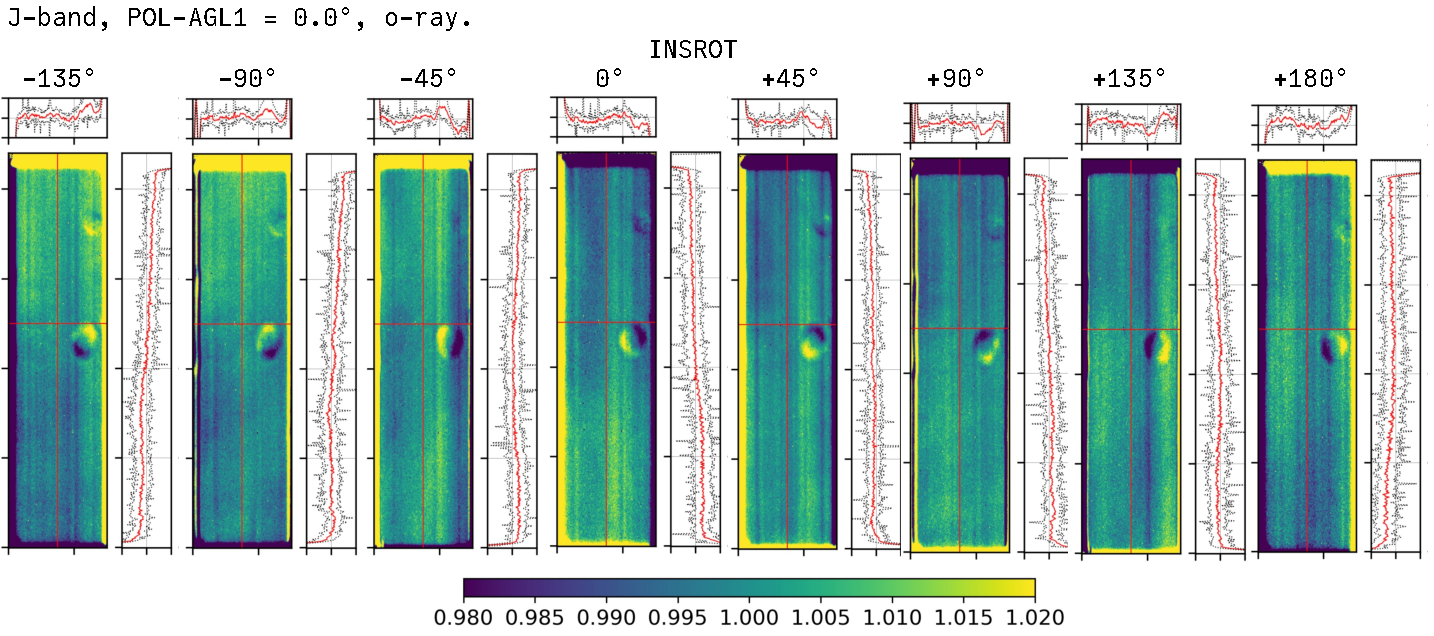
\includegraphics[width=\linewidth]{figs/flatinsrot.pdf}
%   \end{center}
%   \caption[The $ r_1 $ ratio map for J-band with HWP rotator angle $ 0^\circ $ and o-ray region only.]{Explanation, blah blah blah blah blah blah blah blah blah blah blah blah blah blah blah blah. Figure from \cite{2022_SAG_NICpolpy}.}
%   \label{fig:flatinsrot}
% \end{sidewaysfigure}



% \begin{sidewaystable}[!ph]
%   \centering
%   \caption[Symbols frequently used in this paper.]{Explanation blah blah blah blah blah blah blah blah blah blah blah blah blah blah blah blah Table is from \cite{2019JKAS...52...71B}.}
%   \label{tab: notation}
%   \setlength{\tabcolsep}{19pt}
%   \begin{tabular}{llll}
%     \hline\hline
%     Category & Symbols & Description & Value and Unit \\  % Table Heading
%     \hline
%     Magnitudes
%      & $ V_\odot $         & Visual magnitude of the Sun           & $ -26.762 \mathrm{(mag)} $       \\
%      & $ V $, $ \Delta V $ & Visual magnitude and its uncertainty  & $ \mathrm{(mag)} $ \\
%      & $ \HVa $            & Reduced magnitude                     & $ \mathrm{(mag)} $ \\
%      & $ \HV $             & Absolute magnitude ($ \coloneqq \HV(0) $) & $ \mathrm{(mag)} $ \\
%      & $ G $               & Slope parameter                       & ~~ --- \\
%     \hline
%     Ephemerides
%      & $ \rhel $, $ \robs $           & Heliocentric/geocentric distance          & $ \mathrm{m} $ or $ \mathrm{au} $ \\
%      & $ \alpha $                 & Phase angle                               & ($ \mathrm{\degr} $ or $ \mathrm{rad} $) \\
%      & $ t $                      & Time on the target (light-time corrected) & $ \mathrm{s} $ or $ \mathrm{JD} $ \\
%      & $ (\lambda,\, \beta) $     & Ecliptic coordinate (longitude, latitude) & ($ \mathrm{\degr} $ or $ \mathrm{rad} $) \\
% %     & $ (\lambda_\h,\, \beta_\h)_\mathrm{h.e.} $
% %                                  & Heliocentric $ (\lambda, \beta) $         & ($ \mathrm{\degr} $ or $ \mathrm{rad} $) \\
% %     & $ (\lambda_\g,\, \beta_\g)_\mathrm{g.e.} $
% %                                  & Geocentric $ (\lambda, \beta) $           & ($ \mathrm{\degr} $ or $ \mathrm{rad} $) \\
% %    \hline
% %    Rotation
% %     & $ \spin_1 $, $ \spin_2 $
% %                                & Rotational/precessional vector              & ($ \mathrm{\degr} $, $ \mathrm{\degr} $)  \\
% %     & $ P_1 $, $ P_2 $           & Rotational/precessional period            & $ \mathrm{s} $ or $ \mathrm{day} $ \\
% %     & $ \omega_1 $, $ \omega_2 $ & Rotational/precessional angular speed     & $ \mathrm{s^{-1}} $ ($ \mathrm{rad/s} $) \\
% %     & $ \varphi_1 $, $ \varphi_2 $ & Rotational/precessional phase offset    & ($ \mathrm{rad} $) \\
%     \hline
%     Physical
%      & $ S_\mathrm{proj} $      & Total projected area viewed at $ \alpha = 0 $ & $ \mathrm{m^2} $ \\
%     parameters
%      & $ D $           & Effective diameter                                   & $ \mathrm{m} $ or $ \km $\\
%      & $ \pV $         & Geometric albedo in visual (V) band                  & ~~ --- \\
%      & $ A_5 $         & Albedo at the phase angle of $ \alpha = 5 \degr $    & ~~ --- \\
%      & $ I $           & The irradiance of the object of interest             & $ \mathrm{W/m^2} $ \\
%      & $ F $           & $ I $ of a Lambertian reflector at normal incidence  & $ \mathrm{W/m^2} $ \\
%      & $ I/F $         & The radiance factor                                  & ~~ --- \\
%     \hline
%   \end{tabular}
% \end{sidewaystable}

 % ch-theo : Figure and Table tex 파일인 듯, 추후 수정 요망

% ------------ Reference and Code ------------ %
\chapter{Background}
% \chapquote{He integrates empirically.}{Albert Einstein, {\footnotesize after saying ``God does not care about our mathematical difficulties.''}}
% \theoremstyle{definition}


본 연구의 연구 흐름에 대해 기술하는 장이다. motivation부터 연구를 이해하는데 필요한 배경 지식, 본 연구의 필요성 등이 논리적으로 함유되었다.

\section{NeRF and QRF}
% \subsection{NeRF and QRF}
% \textit{설명(삭제예정) : 컴퓨터 비전(상당히 대중적인 주제)의 문제로부터 양자머신러닝 모델의 잠재력을 어필하는 장이다.}

% 컴퓨터 비전 분야에서, 특정 객체에 대한 여러 사진을 Input으로 하여, 입력되지 않은 새로운 view에서의 객체의 형상을 모델링하는 task는 굉장히 중요한 문제이다. view synthesis라고 불리는 이 작업은, 기존에는 해당 객체를 포함한 공간(보통은 3D)의 정보를 모두 픽셀 단위로 저장하고, 이를 원하는 때에 알맞게 load하여 모델링하는 방식으로 이루어졌으나, 해상도가 높아짐에 따라 저장해야 하는 정보가 과도하게 많아진다는 문제가 있었다. 따라서 이를 효율화하기 위한 시도가 계속해서 존재했고, 대표적으로 NeRF(Neural Radiance Field)가 보다 효율적이고 안정적인 대체제가 되었다.
% NeRF 설명 ~~
% 그런데, NeRF 또한 이러이러한 단점이 존재했고, 이를 보완한 QRF(Quantum Radiance Field)가 대두되었다.

MLP(Multi-Layer Perceptron, 다층 퍼셉트론)는 머신러닝에서 사용되는 기본적인 모델로, 여러 분야에서 널리 사용되고 있다. 특히 컴퓨터비전 분야에서 중요한 작업인 3D view synthesis에서, NeRF(Neural Radiance Field)라는 기법이 MLP 모델을 사용하여 두드러진 성과를 보였다. NeRF가 3D view synthesis를 수행하는 방식은 다음과 같다. 먼저 3D 객체를 보는 방향 \( (\theta, \pi)  \in \mathbb{R}^2\)과 그 방향에 놓인 위치 좌표 $(x,y,z) \in \mathbb{R}^3$에 대한 정보가 주어졌을 때, MLP를 사용하여 $\text{color 정보 }(r,g,b) \in \mathbb{R}^3$ 를 예측한다. 이렇게 예측한 color값들은 volume rendering(이산 적분)을 통해, 특정 카메라 위치에서 바라본 이미지의 최종 color값을 예측하는 데 사용된다. 즉, 이산적인 2D view 이미지 데이터를 통해 학습하여, 연속적인 view에 대해서 이미지를 렌더링 할 수 있게 된다. 이러한 방법은 view에 대해 색상 값을 효과적으로 생성하면서도 낮은 저장 공간 요구와 빠른 추론 시간을 유지하기 때문에 많은 관심을 받았다.

 그러나 NeRF는 MLP 구조에 의존하고 있어 속도와 효율성 측면에서 한계가 있다. 최근 문헌에서는 NeRF의 머신러닝 과정을 양자컴퓨팅으로 대체하면 속도와 성능이 향상될 수 있다는 주장이 제기되었다. 이러한 제안은 QRF(Quantum Radiance Field) 연구에서 강조되며, NeRF 프레임워크에 양자 머신러닝을 통합함으로써 현재의 제약을 극복할 수 있는 잠재적 이점에 대해 논의하고 있다.

QRF는 NeRF에서의 ML 모델을 PQC(Parameterized Quantum Circuit) 모델로 대체한 것으로, 큰 차원의 데이터를 양자 데이터로 인코딩함에 따라 데이터의 규모를 축소하고, 이를 통해 resource와 연산 측면의 이득을 취하였다(고 주장한다). 그러나 QRF를 제안한 논문에서는 성능이 왜 개선되었는가에 대한 수학적 근거가 제시되지 않았다. 이에 우리는 궁극적으로 QRF가 실제로 작동하는지, 작동한다면 왜 좋은 결과를 나타내는지에 대해 의문을 갖고, NeRF와 QRF의 핵심인 ML과 QML 차원에서의 수학적인 비교 분석을 하게 되었다.

% 이에 우리는 이 방법론이 실제로 작동하는지, 작동하면 왜 좋은 결과를 나타내는지 수학적으로 분석하고자 하였다.
% 속도가 왜 빨라졌는지, 정확성이 왜 높아졌는지에
% ==> 우리가 이 연구를 시작하게 되었다. 먼저 얘는 ML, QML의 차이이기 때문에 ML, QML의 분석이 선행되었다.

% \subsection{ML and QML}\label{ss:ml and qml}
% 설명(삭제예정) : QRF로 설득한 QML의 잠재력을 가지고 ML과 QML의 공통점/차이점, QML의 필요성 등을 더 설명하는 장이다. 사실 3.1.1만 있으면 좀 부실해보여서 넣는 장이긴 함
% QML의 연구가치, 적용 가능해 보이는 분야들 -> 진짜 motivation이 될 수 있을 법한 내용들

% 이처럼
% 양자 머신러닝은 기존 머신러닝의 한계를 극복하는 데 효용이 있을 것으로 기대되어 활발히 연구 중인 주제이며, ML과 QML의 대표적인 공통점과 차이점은 다음과 같다.

% 공통점으로는, 전체 구조적으로 동일한 양상을 띈다는 것이 있다. ML과 QML 모두 데이터를 Encoding하고, 문제에 맞게 구성된 모델을 통해 output을 내놓는다. 이렇게 얻은 output을 통해 미리 정의된 cost function의 출력값을 계산하고, 계산된 cost 값을 최소화하도록 학습이 진행된다.

% ML과 QML의 가장 큰 차이점은, QML 모델은 데이터 인코딩부터 output 값을 생성하는데까지의 과정이 양자 컴퓨터 상의 양자 알고리즘으로 이루어진다는 것이다. QML 모델은 후술할 여러 방법들을 통해 가지고 있던 기존의 데이터를 중첩시킨 양자 데이터로 변환하고, 양자 회로로 이루어진 Ansatz를 통해 output을 내놓게 된다. 대부분의 QML에서, 이후의 optimize 과정은 고전 ML과 동일하다.

% QML은 양자 컴퓨터에서 작동하는 양자 알고리즘의 이점을 활용하고자 하며, 다양한 방법을 통해 다양한 분야로 적용하려 하는 시도들이 행해지고 있다. 이에 양자 머신러닝의 근간이 되는 양자컴퓨팅의 수학적 이론부터, 양자 머신러닝이 행해지는 방법과 원리를 이해하고 이를 분석해보았다.


%#########################################################
% 3.3 Quantum Machine Learning
%
% Author : SEHYUN YUK
% Last Update: 2024.12.08
%
%##########################################################
\section{Implementations and Experiments} \label{qml:comparision}

 이 절에서는 우리의 본래 목적인, QRF에서 사용된 QML의 세부 요소를 설명한다. 또한 두 가지 문제에 대해 ML과 QML 모델을 각각 구현하여 실제 ML과 QML의 결과값을 비교 분석해보고자 한다.


% 이 절은 우리의 본래 목적인 실험적으로 드러나는 QML과 ML의 차이를 수학적으로 보이는 절이다.
공평한 비교를 위해 똑같은 데이터를 사용하고, 똑같은 파라미터의 개수를 사용하였을 때, 특정함수를 추정하는 Task에서의 성능차이를 보이고자 하였다. 먼저 QRF논문에서 사용된 2d image를 reconstruction 하는 Task에서 작동방식을 확인하고, 이를 더 확실하게 검증하기 위해 1차원 함수를 추정하는 Task에서 또한 검증을 추가적으로 진행하였다.
\begin{itemize}
    \item \textbf{2d image reconstruction} :

        본 태스크는 xy 좌표를 입력으로 받아 RGB 값의 3차원을 예측하는 문제이다. 모델은 각 좌표 \((x, y)\)에 대해 색상 벡터 \((r, g, b)\)를 예측하며, 예측된 색상과 실제 색상 간의 손실을 계산하여 학습을 진행한다. 이를 수식으로 표현하면 다음과 같다.

            \[
            \text{Input}: \mathbf{p} = (x, y) \in \mathbb{R}^2
            \]

            \[
            \text{Prediction}: \hat{\mathbf{c}} = (\hat{r}, \hat{g}, \hat{b}) = f(\mathbf{p}; \theta)
            \]

            \[
            \text{Loss Function}: \mathcal{L}(\theta) = \frac{1}{N} \sum_{i=1}^{N} \| \hat{\mathbf{c}}_i - \mathbf{c}_i \|_2^2
            \]




            여기서 \(f\)는 모델 함수, \(\theta\)는 모델의 파라미터, \(N\)은 데이터 샘플의 수를 나타낸다. 모델은 손실 함수를 최소화하도록 파라미터 \(\theta\)를 최적화하여 예측된 RGB 값이 실제 값과 잘 일치하도록 학습된다. 여기서 ML과 QML의 차이는 모델과 데이터 인코딩에서만 차이나는데, 각각 다음과 같이 진행된다.


              \begin{table}[ht]
                    \centering
                    \begin{tabular}{ l||p{5.5cm}||p{5.5cm}}
                    \Xhline{3\arrayrulewidth}
                    \textbf{Item} & \textbf{MLP} & \textbf{QML} \\
                    \hline
                    Data Encoding & $(x,y) \in \mathbb{R}^2$을 $[-1 ,1]$ 사이로 정규화 하였다.    &
                    Angle Encoding을 사용하였다.$(x,y) \in \mathbb{R}^2$을 $[-1 ,1]$ 사이로 정규화한 이후 이 두 값을 3 개의 qubit 중 두개의 quibt에 RX gate에 $\theta_x ,\theta_y  $들을 각각 $ [-\pi ,\pi]$ 값 사이에 위치하도록 정규화하여  Angle encdoing 하였다.
                     \\
                    \hline
                    Model & MLP 모델을 사용하였으며, 입력에이어 1개 , 히든 레이어 1개 ,출력 레이어 1개로 구성하였으며, activation function은 RELU를 사용하였다. &
                    QRF에서 사용된 PQC 모델과 동일하도록 사용하였다. 총 3개의 qubit을 사용하였고, $ \prod_{0}^{2} RY_i(\theta)CX_i$ 의 gate를 3번 반복함으로써 3층의 레이어의 효과가 나타나도록 구현하였다. 이를 시각화면 다음과 같다.\labelcref{fig:2d-image}
                     \\
                    \Xhline{3\arrayrulewidth}
                    \end{tabular}
                    \caption{MLP와 QML의 비교}
                    \label{tab:mlp_qml_comparison}
                \end{table}

                % \clearpage
                \begin{figure}[h]
                    \centering
                    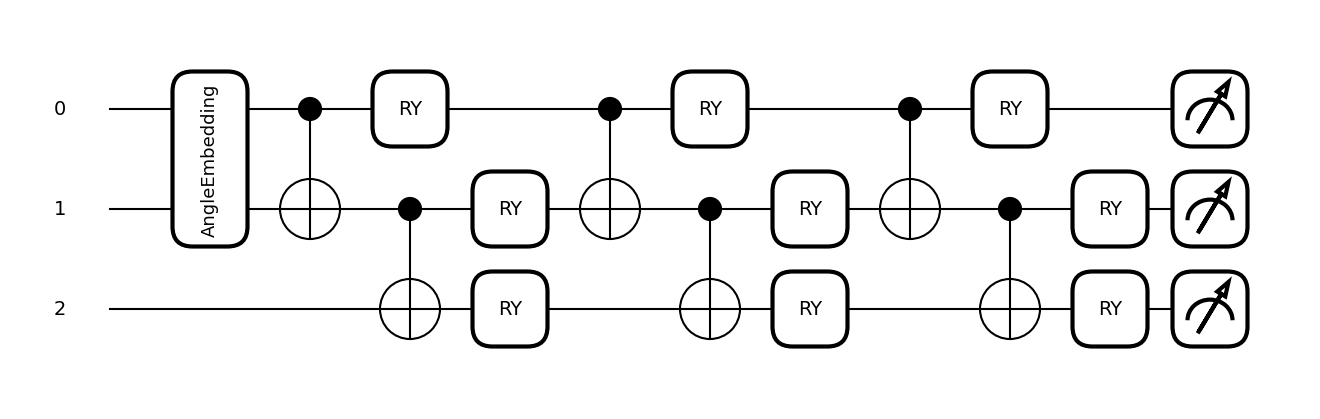
\includegraphics[width=0.8\textwidth]{figs/pqc_2d}\
                \caption{2-d image quantum circuit 구조}
                \label{fig:2d-image}
                \end{figure}

                이러한 모델은, 우리는 사진 3장(256x256)에 대하여, reconstruction error를 PSNR metric를 사용하여 학습된 성능을 평가하였다. PSNR의 수식은 다음과 같이 정의 된다.이는 높은 PSNR이 더 잘 reconstruction함을 뜻한다.

                \[
                    \text{PSNR} = 10 \cdot \log_{10}\left(\frac{\text{MAX}_I^2}{\text{MSE}}\right)
                    \]

                이와 같은 방법으로, 여러 layer별로 성능차이를 비교해보았으며, 결과는 다음과 같이 나타났다.

                \begin{table}[ht]
                    \centering
                    \begin{tabular}{c|ccc}
                    \Xhline{3\arrayrulewidth}
                    \multirow{2}{*}{Layers} & \multicolumn{3}{c}{PSNR (dB)} \\
                    \cline{2-4}
                    & Image 1 & Image 2 & Image 3 \\
                    \hline
                    MLP (3 layers) & 15.826 & 16.913 & 15.884 \\
                    MLP (4 layers) & 15.816 & 17.049 & 16.328 \\
                    MLP (5 layers) & 15.811 & 16.606 & 16.306 \\
                    \hline
                    PQC (3 layers) & 14.503 & 16.269 & 15.470 \\
                    PQC (4 layers) & 15.624 & 16.464 & 15.471 \\
                    PQC (5 layers) & 4.484 & 6.912 & 8.786 \\

                    \Xhline{3\arrayrulewidth}
                    \end{tabular}
                    \caption{PSNR comparison between MLP and QML models across different layer configurations}
                    \label{tab:psnr_comparison}
                \end{table}

        \item \textbf{1-d function estimation} :
본 태스크는 1차원 입력 x를 받아 스칼라 값 y를 예측하는 문제이다. 모델은 입력 x에 대해 출력 y를 예측하며, 예측된 값과 실제 값 간의 손실을 계산하여 학습을 진행한다. 이를 수식으로 표현하면 다음과 같다:

\[
\text{Input}: x \in \mathbb{R}
\]

\[
\text{Prediction}: \hat{y} = f(x; \theta)
\]

\[
\text{Loss Function}: \mathcal{L}(\theta) = \frac{1}{N} \sum_{i=1}^{N} (\hat{y}_i - y_i)^2
\]

여기서 \(f\)는 모델 함수, \(\theta\)는 모델의 파라미터, \(N\)은 데이터 샘플의 수를 나타낸다. 모델은 손실 함수를 최소화하도록 파라미터 \(\theta\)를 최적화하여 예측된 값이 실제 값과 잘 일치하도록 학습된다. ML과 QML의 차이는 모델과 데이터 인코딩에서만 차이나는데, 각각 다음과 같이 진행된다.


\begin{table}[ht]
    \centering
    \begin{tabular}{ l||p{5.5cm}||p{5.5cm}}
    \Xhline{3\arrayrulewidth}
    \textbf{Item} & \textbf{MLP} & \textbf{QML} \\
    \hline
    Data Encoding & $x \in \mathbb{R}$을 $[-1, 1]$ 사이로 정규화하였다. &
    Angle Encoding을 사용하였다. $x \in \mathbb{R}$을 $[-1, 1]$ 사이로 정규화한 이후, 이 값을 2개의 qubit 중 첫 번째 qubit의 RX gate에 $\theta_x$를 $[-\pi, \pi]$ 값 사이에 위치하도록 정규화하여 Angle encoding 하였다. \\
    \hline
    Model & MLP 모델을 사용하였으며, 입력 레이어 1개, 히든 레이어 1개, 출력 레이어 1개로 구성하였으며, activation function은 RELU를 사용하였다. &
    2개의 qubit을 사용하였고, $\prod_{0}^{1} RY_i(\theta)CX_i$의 gate를 3번 반복함으로써 3층의 레이어의 효과가 나타나도록 구현하였다.이를 다음과 같이 시각화하였다.\labelcref{fig:1d-image} \\
    \Xhline{3\arrayrulewidth}
    \end{tabular}
    \caption{MLP와 QML의 비교}
    \label{tab:mlp_qml_comparison_1d}
\end{table}

\begin{figure}[h]
    \centering
    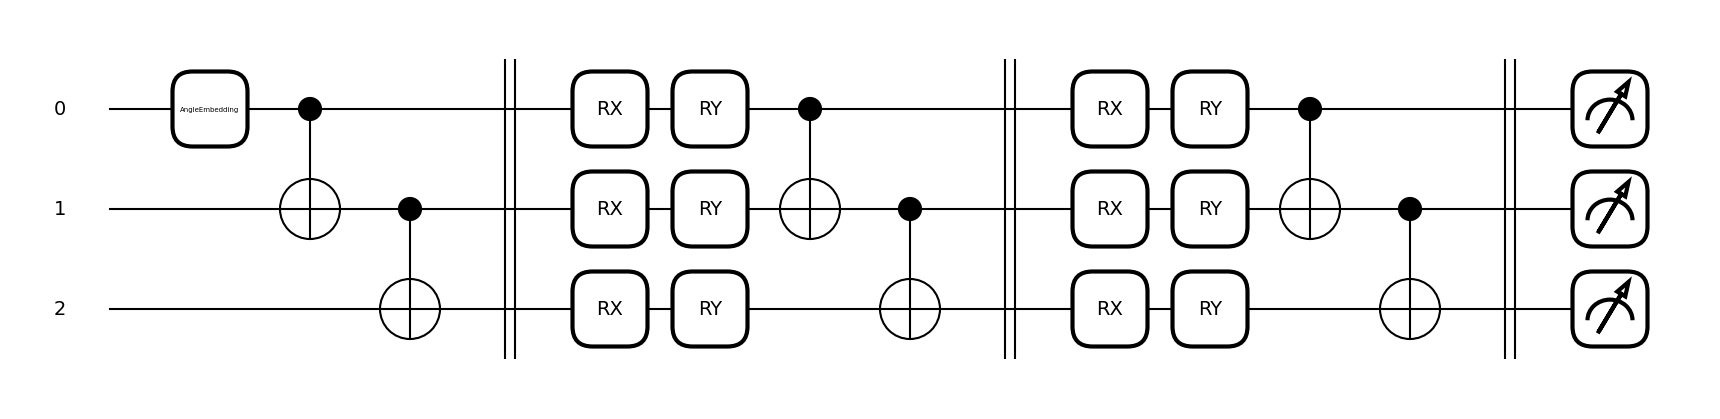
\includegraphics[width=0.8\textwidth]{figs/pqc_1d}\
\caption{1-d function estimation quantum circuit 구조}
\label{fig:1d-image}
\end{figure}
\end{itemize}
\clearpage

이 실험또한 마찬가지로, 여러 레이어의 개수로 실험하였고, 다양성을 위해 3 개의 함수에서 MSE  결과를 측정하였다.

\begin{table}[ht]
    \centering
    \begin{tabular}{c|ccc}
    \Xhline{3\arrayrulewidth}
    \multirow{2}{*}{Layers} & \multicolumn{3}{c}{MSE} \\
    \cline{2-4}
    & $sin(x)$  & $tanh(x)$ & $x$ \\
    \hline
    MLP (3 layers) & 0.0 & 0.0 & 0.0 \\
    MLP (4 layers) & 0.0 & 0.0 & 0.0 \\
    MLP (5 layers) & 0.0 & 0.0 & 0.0 \\
    \hline
    PQC (3 layers) & 0.0 & 0.0 & 0.003 \\
    PQC (4 layers) & 0.0 & 0.0 & 0.003 \\
    PQC (5 layers) & 0.0 & 0.0 & 0.003 \\
    \Xhline{3\arrayrulewidth}
    \end{tabular}
    \caption{MSEcomparison between MLP and QML models across different layer configurations}
    \label{tab:mse_comparison}
\end{table}




\section{Limitations of QML: Constraint of Nonlinearity}

3.3절에서 살펴본 결과, QML이 2d, 1d에서 잘 작동하지 않는 것을 확인하였다. 이에 대한 이유를 quantum circuit의 비선형성의 부족으로 유추하였다. 이를 수학적으로 분석하기 위해, QML의 circuit 구조에 따라, 입력에서 출력까지 나오게 되는 과정을 수식화하였다. \labelcref{fig:1d-image} 와 \labelcref{fig:2d-image}들은 3 qubit cricuit 이므로 gate들의 연산을 모두 $8x8$ 행렬로 나타낼 수 있다. 이러한 행렬의 곱셈연산과 마지막 observable 과정 $ \langle \psi | O | \psi \rangle$ 을 거치면, 마지막 출력 값을 입력에 대한 식으로 표현할 수 있다.  sympy 라이브러리를 통해 식 간략화 및 계산 전개등을 수행하였고 최종식을 도출하였다. 이 식이 정당성에 대한 검증은 실제모델의 값과 비교해봄으로써 확인하였다.

 \labelcref{fig:1d-image} 의 출력을 행렬연산을 통해 도출한 최종값을 수식으로 표현하면 다음과 같이 표현된다.

\begin{equation*}
    y_1  = c_1\cos{\left(x_{1} \right)} - c_2\cos{\left(x_{2} \right)} - c_3\cos{\left(x_{1} - x_{2} \right)} - c_4\cos{\left(x_{1} + x_{2} \right)}
\end{equation*}


\begin{equation*}
y_2  = - c_4\cos{\left(x_{1} \right)} + c_5\cos{\left(x_{2} \right)} - c_6\cos{\left(x_{1} - x_{2} \right)} - c_7\cos{\left(x_{1} + x_{2} \right)} - c_8
\end{equation*}

\begin{equation*}
   y_3 =  -c_9 \cos{\left(x_{1} \right)} + c_{11} \cos{\left(x_{2} \right)} - c_{12} \cos{\left(x_{1} - x_{2} \right)} - c_{13} \cos{\left(x_{1} + x_{2} \right)} - c_{14}
\end{equation*}


여기서 $ c_i $ 들은 PQC의 파라미터에 따라 변하는 값들이며, 매우 복잡한 파라미터값들의 곱 연산을 통해 계산된다. 그러나 최종적으로 파라미터 값이 결정되면 이 값들은 고정되며, $ y_1 ,y_2 , y_3 $ 값들은  $\cos(x_1)$과 $\cos(x_2)$들과 $c_i$ 값들의 linear combination으로 이루어진다. 이를 통해 출력이 선형적이며, 제한된 표현력을 가지고 있음을 관찰하였다.

\clearpage

\labelcref{fig:2d-image}에서 의 출력또한 행렬연산을 통해 최종값을 수식을 도출하였고 이를 수식으로 표현하면 다음과 같다.

\begin{equation*}
 y = - c_1 \sin{\left(x_{1} \right)} - c_2 \cos{\left(x_{1} \right)} + c_3
\end{equation*}

여기서 또한 $c_i$ 값들이 고정되면  $sin(x)$ 와 $cos(x)$ 형태의 linear combination으로 표현되며, 이러한 식은 삼각함수 근사에서만 높은 성능을 보였던 것을 잘 설명해준다. 이러한 선형성은 $\sin(x)$와 $\cos(x)$ 에 대해서만 표현되는 제한적인 표현력을 보여주며, 다양한 함수를 근사하기 위해서는 반드시 비선형성이 필요하다는 것을 시사한다.

 % 3장 tex 파일

% ------------ Part 2 표지 ------------ %
\part{Research and Results}\label{part-conclusion}

% ------------ Chapter 4 시작 ------------ %
\chapter{Research}\label{c:researsh}
% \section{Quantum Perceptron with Quantum Activation Function}
우리는 양자 머신러닝의 큰 진입장벽 중 하나가 비선형성의 구현이라는 것을 이전 장에서 발견했다.
양자 알고리즘의 각 step, 즉 각 게이트를 통과하는 프로세스 하나하나는 모두 각 게이트에 대응되는 행렬을 벡터에 곱해 주는 작업으로 환원된다. 
행렬곱은 본질적으로 선형 연산이므로, 결국 양자 알고리즘으로 완전한 비선형성의 구현이 불가능하다는 결론에 이르게 된다.
인공지능, 그중에서도 MLP(Multi Layer Perceptron)는 행렬 연산의 반복으로 구성되는데, 행렬 연산의 차원을 높이기 위해 각 Layer 사이에 비선형 연산을 추가하는 것이 필수적이라는 사실을 생각하자.
해당 문제의 해결이 선행되기 전까지 MLP를 양자 알고리즘만으로 완전히 구현하는 것은 불가능하다는 것을 어렵지 않게 떠올릴 수 있다.
그렇기에 고전 알고리즘과 양자 알고리즘을 적절히 섞어 사용하는 Hybrid Algorithm이라는 시도가 있다. 하지만 양자 알고리즘만으로 머신 러닝의 과정을 모두 구현하겠다는 시도는 분명 학술적으로 그 가치가 충분하다.

우리는 상기한 문제의 해결 방법을 제시한 논문을 발견하였다.
해당 논문에는 단층 퍼셉트론의 연산 프로세스를 양자 회로로 구현하는 방법이 제시되어 있다.
단층 퍼셉트론은 크게 \(N_{in} \times 1\) 크기의 input vector \(\vec{x}\), 
\(\vec{x}\)의 각 성분과 곱해지게 될 가중치 값이 저장되어 있는 \(N_{in} \times 1\) 크기의 weight vector \(\vec{w}\), 
스칼라 값인 bias \(b\), 그리고 비선형성을 위한 활성화 함수(Activation Function, AF) \(f\)로 구성되어,
\(\vec{x}\)가 input으로 주어지면 \(f(\vec{w}\cdot\vec{x}+b)\)의 값을 내놓는다.
해당 논문은 \(\vec{w}\cdot\vec{x}+b\)의 계산뿐만 아니라, \(f(\vec{w}\cdot\vec{x}+b)\)의 계산 또한 양자 알고리즘으로 구현한다.

우리는 해당 논문을 이후 연구의 중심 축으로 결정하였다.
우리는 해당 논문을 이해하고, 수학적 과정을 코드로 구현하여 시각적으로 확인해 보았다.
또한 논문에서는 제대로 논의하고 있지 않은 부분인 MLP의 양자적 구현을 위해 고민하던 중, 우리는 매우 효율적인 Multiperceptron의 양자 알고리즘을 구현하는 데에 성공하였고, 이를 코드로 구현하여 잘 작동함을 확인하였다.

이번 장은 해당 논문에 대한 우리의 심도 깊은 이해와 구현, 그리고 우리가 발전시킨 부분에 대해 서술되어 있다.
4.1장에서는 \(f(\vec{w}\cdot\vec{x}+b)\)를 양자 알고리즘으로 구현하는 과정을 따라가고, 그 과정을 직접 코드로 구현해 본 과정을 공유한다.
이후 4.2장에서는 우리의 독창적이고 효율적인 Multiperceptron의 구현 과정을 설명한다.

\section{Impartion Nonlinearity for Quantum Perceptron}

\subsection{Summarization of the Notations}

이번 Section은 앞으로의 내용을 내용을 잘 이해하기 위해, 기호들이나 용어의 의미를 정리하기 위한 장이다.

앞으로 qubit의 개수를 표기하는 영어 소문자에 대해, 대문자 표기는 그 qubit에 대응되는 Hilbert Space의 차원을 나타낸다.
즉 qubit 개수가 n인 경우, N = \(2^n\)이다.

임의의 1개 qubit과 대응되는 2차원 Hilbert Space \(\mathcal{H}\)에 대하여, register q의 n개의 qubit과 대응되는 \(2^n\)차원 힐베르트 공간을 \(\mathcal{H}_q^{\otimes n} \equiv \mathcal{H}_{q_{n-1}} \otimes \mathcal{H}_{q_{n-2}} \otimes \dots \otimes \mathcal{H}_{q_{0}}\) 라고 한다.
이때 register는 qubit이 저장되어 있는 공간의 이름을 말한다. 간단하게 이해하면 qubit의 집합이라고 생각하면 된다.
\(\mathcal{H}\)의 computational basis가 \(\{ \ket{0}, \ket{1} \}\)임을 일전에 이야기했다. 그렇기에 \(\mathcal{H}_q^{\otimes n}\)의 computational basis는 \(\{ \ket{s_{n-1}s_{n-2}\dots s_0} : s_k \in \{0,1\}, k = 0,1,\dots , n-1\}\)의 이진수 형태로 나타내어지고, 각 원소는 이를 십진수 형태로 변환한 \(\{ \ket{i}, i \in \{0,1,\dots,2^n-1\} \} \)의 형태로 나타낼 수도 있다.
예컨대, \(\ket{N-1} \equiv \ket{2^n-1} \equiv \ket{111\dots 1} \equiv \ket{1}^{\otimes n}\)가 된다.

n개의 qubit으로 구성된 register q에 적용되는 연산 U를 표기하는 방법은, U가 separable인지 아닌지에 따라 나뉜다.
sperable이 아닌 경우에는 U가 q에 가해지는 연산임을 나타내기 위해 \(U_q\)라고 작성하거나, 아니면 단순히 U라고 적는다.
한편, U가 one-qubit transformation \(U_{q_j}\)들의 텐서곱으로 나타내어지는, 즉 separable인 경우에는 U를 \(U_q^{\otimes n} \equiv U_{q_{n-1}} \otimes U_{q_{n-2}} \otimes \dots \otimes U_{q_{0}}\)라고 적는다.

n개의 qubit으로 구성된 register q, d개의 qubit으로 구성된 register a를 생각하자. 두 레지스터는 N+D차원 Hibert Space로 합쳐질 수 있다. 이 합쳐진 Space를 \(\mathcal{H}_a^{\otimes d} \otimes \mathcal{H}_q^{\otimes n}\)로 작성한다. 이때 이 Space의 computational basis는 \(\{ \ket{i}_a \ket{j}_q : i = 0,\dots,D-1, j = 0,\dots,N-1\}\)이다.
간결함을 위해, 연산 O가 만약 둘 중 하나의 register에서만 작동하는 경우에 \(\mathbb{1}_a \otimes O_q, O_a \otimes \mathbb{1}_q\)를 각각 \(O_q, O_a\)로 간단하게 나타낸다. 이때 \(\mathbb{1}_a = I_{2^d}\)를 의미한다.
특히, \(\ket{i}\bra{i}_q \equiv \mathbb{1}_a \otimes \ket{i}_q {_q}\bra{i}\)는 register q의 \(\ket{i}\) state로의 D차원 projection을 나타낸다.

마지막으로, controlled gate(특정 qubit의 상태에 따라 연산의 작동 여부가 결정되는 게이트)를 나타내기 위해 사용하는 표기들을 정리해 보자. \(C_{q_i}U_{q_j}\)라는 표기는 \(q_i\) qubit의 state가 \(\ket{1}\)일 때 \(q_j\) qubit에 연산 U를 가하겠다는 의미이다.
이와 반대로 \(\bar{C_{q_i}}U_{q_j}\)은 \(q_i\) qubit의 state가 \(\ket{0}\)일 때 \(q_j\) qubit에 연산 U를 가하겠다는 의미이다.
즉 \(\bar{C_{q_i}}U_{q_j}\)은 \(X_{q_i}C_{q_i}U_{q_j}X_{q_i}\)와 동일한 연산이다. (X: Pauli-X gate)
만약 d개의 qubit으로 구성된 register a의 모든 qubit을 control qubit으로 사용하는 경우에는 \(C_a^dU_{q_j}\)라는 표기를 사용한다.

\subsection{Implementation of \(\vec{w}\cdot\vec{x}+b\)}

단일 퍼셉트론의 구현을 위해 n+d개의 qubit이 필요하다. n개의 qubit은 q register에, d개의 qubit은 a register에 들어 있다. input vector \(\vec{x}\)의 크기는 \(N_{in}\)으로 쓴다.
우선은 각 input값을 scaling하여 각 성분을 -1과 1 사이의 값으로 고정시키는 것으로 시작한다.
즉, \(\vec{w} \in [-1,1]^{N_{in}}, \vec{x} \in [-1,1]^{N_{in}}, b \in [-1,1]\)이 주어졌을 때, \(\vec{w}\cdot\vec{x}+b\)의 값을 계산하는 양자 회로의 구성 과정을 따라가 보겠다.

\begin{lemma}
    \(\vec{x}, \vec{w}, b\) 가 주어졌을 때, \(\displaystyle \bra{N-1}U_z(\vec{x},\vec{w},b)\ket{0} = \frac{\vec{x}\cdot \vec{w}+b}{N_{in}+1} \equiv z\) 를 만족하는 Unitary transformation \(U_z(\vec{x},\vec{w},b)\) 의 역할을 하는 양자 회로를 만들 수 있다.
\end{lemma}

\begin{pf}(sketch)

Lemma에서 \(\ket{0}, \ket{N-1}\)은 각각 \(\ket{0}^{\otimes n}, \ket{1}^{\otimes n}\)임을 기억하자.
\(\vec{v}_x = (\vec{x},1,A_x,\vec{0}), \vec{v}_{w,b} = (\vec{w},b,\vec{0},A_{w,b})\) 를 만들자.
이때 두 벡터는 \(n = \lceil\log_2{N_{in}+3}\rceil\)에 대해 \(N = 2^n\)의 크기를 가진다. 벡터의 성분으로 들어 있는 0의 개수는 N과 \(N_{in}\)값에 따라 결정된다.
또한, 두 벡터는 \(|\vec{v}_x| = |\vec{v}_{w,b}| = \sqrt{N_{in}+1}\)를 만족해야만 한다. \(A_x, A_{w,b}\)의 값은 해당 규칙에 맞게 결정해 주면 된다.
그러면 \(\vec{v}_{w,b}^T\vec{v}_{x} = \vec{w}\cdot\vec{x}+b \in [-N_{in}-1, N_{in}+1]\)이 자연스럽게 도출된다.

%두 개의 state \(\ket{\psi_{x}},\ket{\psi_{w,b}}\)를 각각 \(\ket{\psi_{x}} = \sum_{i=0}^{N-1}\frac{v_{x,i}}{\sqrt{N_{in}+1}}\ket{i}, \ket{\psi_{w,b}} = \sum_{i=0}^{N-1}\frac{v_{w,b,i}}{\sqrt{N_{in}+1}}\ket{i}\)라 정의하자.
%그러면 \(\bra{\psi_x}\ket{\psi_{w,b}} = \frac{\vec{w}\cdot\vec{x}+b}{N_{in}+1} \equiv z\)가 성립한다.

위에서 만든 두 벡터 \(\vec{v}_x, \vec{v}_{w,b}\)로 \(\bra{\psi_x}\ket{\psi_{w,b}} = \frac{\vec{w}\cdot\vec{x}+b}{N_{in}+1} \equiv z\)가 성립하는 두 개의 state \(\ket{\psi_{x}},\ket{\psi_{w,b}}\)를 만들 수 있다.

\(U_x = \mathcal{U}(\vec{v}_x), U_{w,b} = X^{\otimes n}, \mathcal{U}^\dag(\vec{v}_{w,b})\)라고 작성할 수 있다.
이때 \(\bra{\psi_{w,b}}\ket{\psi_x} = \bra{\psi_{w,b}}U_{w,b}^{\dag} U_{w,b}\ket{\psi_x} = \bra{N-1}U_{w,b}U_x\ket{0}^{\otimes n}\)이 성립하므로, Lemma에서 말하는 \(U_z(\vec{x},\vec{w},b)\)가 \(U_{w,b}U_x = X^{\otimes n}\mathcal{U}^\dag (\vec{v}_{w,b})\mathcal{U}(\vec{v}_x)\)임을 확인할 수 있고, 이것으로 증명이 완료된다.
\end{pf}

\begin{theorem}
    \(\vec{x}, \vec{w},b,z, N\) 에 대하여, 초기에 \(\ket{0}, \ket{0}_q\)로 초기화되어 있는 두 state vector를 (n+d) qubit으로 구성된\(\ket{\psi_z^d}_q = \ket{\psi_z^d}_\perp + \frac{1}{2^{d/2}}\ket{z}_a^{\otimes d}\ket{N-1}_q \in \mathcal{H}_a^{\otimes d} \otimes \mathcal{H}_q^{\otimes n} \)로 변환하는 양자 회로를 구성할 수 있다.
    이때 \(\ket{\psi_z^d}_q\)는 \(\ket{N-1} \bra{N-1}_q\ket{\psi_z^d}_\perp = 0, \ket{z} \equiv \ket{0}+z\ket{1}\)를 만족한다.
    우리가 원하는 양자 회로는 \(S_VX_q^{\otimes n}\)으로, \(V_m = C_{a_m}U_z(\vec{x},\vec{w},b)_qC_{a_m}X_q^{\otimes n}C_q^nH_{a_m}, S_V=V_{d-1}\dots V_1V_0\)을 각각 의미한다.
\end{theorem}

\begin{pf}(sketch)

    이 theorem의 존재 가치는 두 register에 동시에 영향을 끼치는 어떠한 회로를 가지고 우리가 원하는 state \(\ket{\psi_z^d}\)를 얻어낼 수 있음을 보이는 것이다.
    \(\ket{\psi_z^m} \in \mathcal{H}_{a_{m-1}} \otimes \mathcal{H}_{a_{m-2}} \otimes \dots \otimes \mathcal{H}_{a_{0}} \otimes \mathcal{H}_{a}^{\otimes n}\)이라 하자.
    projection 변환 \(\ket{N-1}\bra{N-1}_q\)에 대하여 \(\ket{N-1}\bra{N-1}_q\ket{\psi_z^m}_\perp = 0\)을 만족하도록 \(\ket{\psi_z^m}\)을 \(\ket{\psi_z^m}_\perp + \ket{\psi_z^m}_{||}\)로 분리할 수 있다.
    \(V_m = C_{a_m}U_z(\vec{x},\vec{w},b)_qC_{a_m}X_q^{\otimes n}C_q^nH_{a_m}\)으로 잡을 수 있다. 여기서 \(a_m\)에 의해 작동 여부가 결정되는 \(U_z(\vec{x},\vec{w},b)_q\)는 위의 Lemma에서 결정된 그것이다.
    이제, \(\ket{\psi_z^m}_{||} = \frac{1}{2^{d/2}}\ket{z}_a^{\otimes d}\ket{N-1}_q\)라는 사실을 생각하고, \(V_m\)을 state \(\ket{0}_{a_m}\ket{\psi_z^m} = \ket{0}_{a_m}\ket{\psi_z^m}_\perp + \frac{1}{\sqrt(2)}(\ket{0}_{a_m}+\ket{1}_{a_m})\ket{\psi_z^m}_{||}\)에 적용하여
    \(\ket{\psi_z^{m+1}}\)을 얻게 된다. 이제, 이 과정을 각 qubit에 적용하는 것을 반복하는 연산 \(S_V = V_{d-1}\dots V_1V_0\)을 state \(\ket{0}_a^{\otimes d} \ket{N-1}_q\)에 적용하면, 결과물로 \(\ket{\psi_z^d}\)가 나온다.

\end{pf}


\begin{corollary}
    \(\ket{\psi_z^d}\)에는 \(z^k, (k = 0,1,\dots,d)\) 의 값들이 probability amplitude로 저장되어 있다.
\end{corollary}

\begin{pf}(sketch)
    이상의 Corollary는 위의 Theorem에서 얻은 state \(\ket{\psi_z^d}\)를 measure하지 않고도 z의 값을 사용할 수 있음을 시사한다.
    \(\ket{\psi_z^m}_\perp + \ket{\psi_z^m}_{||}\)라는 사실을 활용하면
    Theorem 1의 식 \(\ket{\psi_z^d}_q = \ket{\psi_z^d}_\perp + \frac{1}{2^{d/2}}\ket{z}_a^{\otimes d}\ket{N-1}_q\)에서 \(_q\bra{N-1}_a\bra{2^k-1}\ket{\psi_z^d} = 2^{-d/2}z^k\) 임을 유도할 수 있다.
\end{pf}

이상으로 첫 번째 단계에 대한 구현 및 증명이 완료되었다. 정리하자면, 논문에서는 \(\ket{\psi_z^d}\)를 얻을 수 있는 양자 회로 \(S_VX_q^{\otimes n}\)의 구조와 그 존재성, 유효성을 수학적으로 증명하였다.
이때 \(\ket{\psi_z^d}\)에는 우리가 원하는 값인 z가 측정의 과정을 거치지 않고도, 즉 양자 회로를 종료할 필요 없이 다음 단계에서 그 값을 활용할 수 있는 형태로 저장되어 있다.

\subsection{Implementation of Activation function}

이제 남은 것은 Activation function의 구현이고, 우리가 핵심적으로 관찰해야 했던 과정이다.
양자 알고리즘으로 \(f(\vec{w}\cdot\vec{x}+b)\)를 구현할 수 있음을 보이고 그 방법론의 타당성을 설명하기 위해서 논문은 크게 두 가지의 단계를 거친다.
우선은 양자 회로로 쉽게 구현할 수 있는 형태의 함수를 결정하고,
어떠한 형태의 함수 f에 대하여, z를 input으로 하면 f(z)의 값을 내놓는 양자 회로를 제시하는 것이다.
그리고 임의의 d차 테일러 전개가 존재하는 함수(analytic 함수)에 대하여, 그 함수의 d차 테일러 전개 \(f_d\)를 일전에 결정한 형태로 작성할 수 있음을 보인다.
a register의 차원 수와 그 양자 회로가 내놓는 f의 taylor expansion의 차수가 동일하다는 사실에 주목하자.
이 과정을 통해 양자 회로로 임의의 analytic 함수의 d차 taylor expansion \(f_d\)에 대하여, \(f_d(z)\)의 값을 양자 회로를 통해 계산할 수 있음을 보이는 방식이다.
각 과정은 이하의 theroem과 corollary로 선언되고, 그 유효성이 증명되어 있다.

\begin{theorem}
    \(\theta_{k} \in [-\frac{\pi}{2},\frac{\pi}{2}], k = 0,\dots,d-1,\)인 \(\theta_{k}\)에 대하여, \(k = 1,\dots,d\)에 대하여 재귀적으로 정의된 함수 \(f_k(z): f_0(z) = 1, f_z(z) = f_{k-1}(z)\cos\theta_{k-1} - z^k\sin\theta_{k-1}\)를 생각하자.
    그러면 \(_a \langle  0|U_k|z \rangle  _a^{\otimes d} = f_k(z)\)를 만족하는 unitary operator \(U_k = C_{a_0}X_{a_k}\bar{C}_{a_k}R_y(-2\theta_{k-1})_{a_0}U_{k-1}, U_0 = \mathbb{1} \) (이 또한 재귀적으로 정의되어 있다)가 존재한다.
\end{theorem}

\begin{pf}(sketch)
    
    2단계의 회로는 \(U_d\)이다. 1단계 과정의 전체 회로를 \(S_VX_q^{\otimes n}\)로 나타내었기 때문에, 표기의 통일성을 위해 전체 회로 그림에서 \(U_d\) 대신 \(S_U\)라는 표기를 사용한다. 둘은 같은 것을 지칭한다.
    

\end{pf}

\begin{corollary}
    임의의 콤팩트한 집합 \(I\)에서 정의된 analytic function \(f\)에 대하여, 위에서 정의된 방식으로 정의한 \(f_d\)가 \(\theta_k\)를 잘 선택하면 실수 \(C_d = \frac{1}{k!}f^{(k)}(0)\prod_{j=k}^{d-1}(\cos\theta_j)^{-1}\)에 대하여 \(C_df_d\)가 \(f\)의 d차 테일러 전개와 같아진다.
\end{corollary}

여기까지 논문에서 제시한 \(f(\vec{w}\cdot\vec{x}+b)\) 계산의 양자 알고리즘 구현 방법이다.
우리는 이 방법론에 대한 수학적 증명 과정을 상세히 이해하였고, 그것의 유효성을 각 theorem을 코드로 구현해 봄으로서 다시 한 번 확인하였다.
f의 구현을 위해 \(\theta_k\)를 계산하고, 이를 양자 회로에 제공하여 \(f(\vec{w}\cdot\vec{x}+b)\)의 값을 출력할 수 있도록 하는 양자 회로의 구현을 최종적으로 완료하였다.

\section{Implementation of Multiperceptron with Superb Efficiency}

지금까지 살펴본 Quantum Perceptron을 제안한 문헌에서는, Quantum Perceptron의 구현이 "임의의 layer 당 neuron 수"와 "임의의 layer 수"에 대한 Quantum-MLP의 구현 가능을 의미한다고 주장한다. 그러나, 이것이 당연한 것은 아니다. 먼저 하나의 layer에 여러 perceptron이 존재하는 경우, 현재까지 구현된 회로를 perceptron의 개수만큼 복사하여 사용하는 것 외에는 특별히 떠오르는 방안이 없다. 심지어 이 방법은 perceptron의 개수가 증가함에 따라 과하게 qubit이 늘어난다는 단점이 있다. 또한, multi-perceptron의 구현 방법이 명확하지 않으므로 layer가 반복될 때의 양자적인 표현도 당연하지 않다.

따라서, 비선형성을 양자적으로 표현한 Quantum Perceptron을 실제로 사용하기 위해서는, 효율적인 multi-perceptron의 구현을 꾀하는 것이 필수적으로 요구된다. 이에 하나의 layer 당 $n$개의 perceptron을 사용하는 multi-percepton을 구현하기 위해 추가로 $\lceil {\log_2(n)} \rceil$만큼의 qubit을 필요로 하는 획기적인 방법을 고안하였고, 이를 소개한다. 
% \subsection{Idea}

핵심 아이디어는, 추가 qubit을 사용해서 여러 weight($\mathbf{w}_1, \mathbf{w}_2, \cdots$)에 대한 state \( \ket{\psi}_{f_d(z_1)}, \ket{\psi}_{f_d(z_2)}, \cdots \)가 중첩된 state를 생성하는 것이다.

% W matrix로? {w_i} 이렇게 집합으로?
\begin{lemma}
% \[
%     \text{Given Input vector } \vec{x} \in [-1, 1]^{N_{in}} \text{, and weight matrix } W := \begin{pmatrix}
%         \vec{w}_0 \\ \vec{w}_1 \\ \vdots \\ \vec{w}_{N_w - 1}
%     \end{pmatrix}\text{, where } \vec{w}_i \in [-1, 1]^{N_{in}} \text{ for } i = 0, 1, \cdots, N_w - 1
% \]
Given Input vector \( \vec{x} \in [-1, 1]^{N_{in}} \), weight matrix \( W:= \begin{pmatrix}
    \vec{w}_0 \\ \vec{w}_1 \\ \vdots \\ \vec{w}_{N_w - 1}
\end{pmatrix} \) , bias vector \( \vec{b} \in [-1, 1]^{N_w} \), and given q-registers s, q with p, n qubit respectively, such that \( n = \left\lceil \log_2(N_{in} + 3) \right\rceil, p = \left\lceil \log_2(N_w) \right\rceil \), then, there exists a quantum circuit \( U_{\mathbf z}(\vec{x}, W, \vec{b}) \) such that 
% \begin{gather*} 
%     \vspace{-1.0em} % 두 수식 간 간격 조정 (값을 조정 가능)
%     \text{Given Input vector } \vec{x} \in [-1, 1]^{N_{in}} \text{, weight matrix } W:= \begin{pmatrix}
%         \vec{w}_0 \\ \vec{w}_1 \\ \vdots \\ \vec{w}_{N_w - 1}
%     \end{pmatrix}\text{, bias vector } \vec{b} \in [-1, 1]^{N_w,} 
%     \\ \vspace{-0.5em}
%     \text{and given q-registers s, q with p, n qubit respectively, such that } n = \left\lceil \log_2(N_{in} + 3) \right\rceil, p = \left\lceil \log_2(N_w) \right\rceil ,
%     \\ \vspace{-0.5em}
%     \text{then, there exists a quantum circuit } U_{\mathbf z}(\vec{x}, W, \vec{b}) \text{ such that }
% \end{gather*}
\[
    {}_{s}\langle{i}| {}_{q}\langle N-1|U_{\mathbf z}(\vec{x}, W, \vec{b})\ket{0}_q \ket{0}_s = {\vec{w}_i \cdot {\vec{x} + 1} \over {N_{in} + 1}} \equiv {z_i \over {{2^{p/2}}}} \quad \text{ for } i = 0, 1, \cdots , N_{w} - 1
\]
\begin{gather*}
    \text{where } \ket{0}_q \equiv \ket{0}^{\otimes n}, \ket{0}_s \equiv \ket{0}^{\otimes p}, \ket{N-1}_q \equiv \ket{1}^{\otimes n},\text{ and } \vec{w}_i \in [-1, 1]^{N_{in}} \text{ for } i = 0, 1, \cdots, N_w - 1
% \vspace{-0.5em} % 두 수식 간 간격 조정 (값을 조정 가능)
\end{gather*}

\end{lemma}

Lemma 4.2.1은, 보유한 각 \(\vec{w}_i\)에 대한 \(\displaystyle {z}_i\) 값 정보를 담는 모든 \(\ket{\psi_{z_i}}\) state가 동일한 확률 \(\displaystyle {1 \over {2^{p/2}}}\)로 중첩되어 있는 state \(\ket{\psi_{\mathbf z}}\)를 만드는 Unitary가 존재함을 의미한다. 증명은 다음과 같다.

\begin{pf} 
    Lemma 4.1.1에 의해, 주어진 weight vector $\vec{w} \in \mathbb{R}^{N_{in}}$와 bias 값 b, \(n = \left\lceil \log_2{N_{in}} + 3 \right\rceil\)개의 qubit에 대해 \(\displaystyle \bra{N-1}U_z(\vec{x},\vec{w},b)\ket{0} = \frac{\vec{x}\cdot \vec{w}+b}{N_{in}+1} \equiv z\)를 만족하는 Unitary transformation \(U_{\mathbf z}(\vec{x},\vec{w},b)\)가 존재한다. 따라서, $n$개의 qubit을 갖는 $q$ register에서 하나의 weight vector와 bias b에 대해 동일한 작업이 가능하다.

    $s$ 레지스터는 weight의 개수 \(N_w\)에 대해, \(p = \left\lceil \log_2(N_w) \right\rceil\)만큼의 qubit을 보유하며, 즉 basis state로 \(\ket{0}, \cdots, \ket{P-1}\)를 가진다.

    이에 따라, \(s\) 레지스터의 \(i\)번째 basis state인 \(\ket{i}\)와, \(q\) 레지스터에서 \(i\)번째 weight vector 및 bias 값에 대한 \(U_z(\vec{x}, \vec{w}_i, b_i)\)의 output state \(\ket{\psi_{z_i}}\)의 텐서곱이 중첩된 state를 만드는 양자 회로를 다음과 같이 설계할 수 있다.
    \[
        U_{\mathbf z}(\vec{x}, W, \vec{b}) = S_{\mathbf z}(\vec{x}, W, \vec{b}) H_s^{\otimes p} \quad \text{ where } S_{\mathbf z}(\vec{x}, W, \vec{b})= \left(\prod_{k=0}^{N_w-1}C_{s}^{ctrl : k}U_{z_k}(\vec{x}, \vec{w}_k, b_k)\right)
    \]
    여기에서 \(C_{s}^{ctrl:k}U_{z_k}(\vec{x}, \vec{w}_k, b_k)\)는 \(s\) 레지스터의 상태가 \(k\)의 이진 표현과 같은 경우, \(q\) 레지스터에 \(U_{z_k}(\vec{x}, \vec{w}_k, b_k)\) 연산을 작동시키는 Controlled-Gate이다.

    이 회로는 먼저 \(s\) 레지스터의 모든 qubit에 Hadamard 연산을 작동시켜 모든 basis state이 동일한 확률로 중첩된 state \(\displaystyle \sum_{i=0}^{P-1} {1\over {2^{p/2}}}\ket{i}\)를 생성한다. 이렇게 생성된 state의 각 basis state는 \(C_{s}^{ctrl:k}U_{z_k}(\vec{x}, \vec{w}_k, b_k)\)에 의해 basis의 이진 표현에 해당하는 $\ket{\psi_k}$와 결부되어, 결과적으로는 다음과 같은 state를 만들게 된다:
    \[
        \ket{\psi_{\mathbf{z}}} := \sum_{i=0}^{P-1} {1\over {2^{p/2}}} \ket{\psi_{z_i}}_q \ket{i}_s 
    \]
    where \(\ket{\psi_{z_i}}_q = \ket{0}_q \text{ for } i \ge N_w\) \quad $\square$
\end{pf}

Lemma 4.2.1에 의해, 4.1절에서와 같은 방식으로 중첩된 state \(\ket{\psi_{\mathbf z}}\)를 사용할 수 있다. 이는 Thm 4.1.1에도 동일하게 적용된다. 다음 Thm을 살펴보자.

\begin{theorem}
    Let \(z_i := \left( \vec{w}_i \cdot \vec{x} + b_i \right) / \left( N_{in} + 1 \right)\) where \(\vec{x}, \vec{w}_i \in [-1, 1]^{N_{in}}\) and \(b_i \in [-1, 1]\) for \(i = 0, \cdots, N_w - 1\). Let $q, a, \text{and} s$ be quantum registers of $n, d, \text{ and } p$ qubits respectively, with \( N = 2^n \ge N_{in} + 3 \) and \( p = \left\lceil N_{w} \right\rceil\). Then there exist a quantum circuit which transforms the three registers from the initial state \(\ket{0}_s \ket{0}_a \ket{0}_q\) to (p+n+d)-qubit entangled state \(\ket{\psi_{\mathbf z}^d}\) of the form 
    \[
        \ket{\psi_{\mathbf z}^d} = \ket{\psi_{\mathbf z}^d}_{\perp} + {1 \over {2^{(d + p) / 2}}}\sum_{i=0}^{N_w - 1}\left( \ket{i}_{s} \ket{z_i}_{a}^{\otimes d} \ket{N-1}_q \right)
    \]
    where
    \[
        \ket{N-1}\bra{N-1}_q \ket{\psi_z^d}_{\perp} = \mathbf{0}
    \]
    and
    \[
        \ket{z_i} \equiv \ket{0} + z_i\ket{1}
    \]  
    The circuit is expressed by $S_V X_q^{\otimes n} H_s^{\otimes p}$ where X is Pauli-X, H is Hadamard gate and 
    \[
        S_V = V_{d-1} \cdots V_1 V_0
    \]
    with
    \[
        V_m = C_{a_m}S_{\mathbf{z}}(\vec{x}, W, \vec{b})_q C_{a_m}X^{\otimes n}_q C_q^nH_{a_m} \quad \text{ for } m = 0, 1, \dots, d - 1
    \]  
\end{theorem}

Thm 4.2.1이 의미하는 바는, 주어진 input vector \(\vec x\) weight matrix \(W\), bias vector \(\vec b\)에 대해, 모든 \(z_i\)의 정보를 담고 있는 entangled state $\ket{\psi_{\mathbf z}^d}$를 생성하는 Unitary가 존재한다는 것이다. 다음 증명을 살펴보자.

\begin{pf}
% Thm 4.1.1의 증명에 의해, for \(i = 0, \dots, d-1, \quad V_i : \ket{\psi_z^i} \mapsto \ket{\psi_z^{i+1}}\)의 동작을 알 수 있다. 

Thm 4.2.1에 명시된 \(S_V X_q^{\otimes n} H_s^{\otimes p}\)의 경우 $V_0$를 시행하기 전에 \(s\) 레지스터의 모든 qubit에 Hadamard를 가하여, \(s\) 레지스터에는 모든 Computational Basis State가 동일한 확률로 중첩된 state가 저장되어 있고, \(q\) 레지스터의 모든 qubit은 Pauli-X gate를 통해 \(\ket 0\)에서 \(\ket 1\)로 변환한다. 이후 \(V_0, V_1, \cdots, V_{d-1}\)이 실행되는데, $V_m$의 동작은 \(V_m = C_{a_m}S_{\mathbf{z}}(\vec{x}, W, \vec{b})_q C_{a_m}X^{\otimes n}_q C_q^nH_{a_m}\)으로, 세 개의 step으로 이루어진다.

1. \(C_q^nH_{a_m}\) : 즉 q 레지스터의 모든 qubit을 control bit로, \(a_m\) qubit을 target bit로 하는 Controlled-Hadamard 연산을 적용한다.

2. \(C_{a_m}X^{\otimes n}_q\) : \(a_m\)의 state가 \(\ket 1\)인 경우에 \(q\) 레지스터의 모든 qubit에 Pauli-X gate를 적용한다.

3. \(C_{a_m}S_{\mathbf{z}}(\vec{x}, W, \vec{b})_q\) : \(a_m\)의 state가 \(\ket 1\)인 경우에 \(q\) 레지스터에 대해 \(S_{\mathbf{z}}(\vec{x}, W, \vec{b})_q\)를 적용한다.

1번째와 2번째 step의 경우 Thm 4.1.2와 동일하다. 3번째 step의 동작을 살펴보면, \(S_V X_q^{\otimes n} H_s^{\otimes p}\)의 첫 동작인 \(H_s^{\otimes p}\)에 의해 \(s\) 레지스터에 동일한 확률 \(1 \over {2^{p/2}}\)로 중첩되어 있는 Basis State와 \(S_{\mathbf z}(\vec{x}, W, \vec{b})= \left(\prod_{k=0}^{N_w-1}C_{s}^{ctrl : k}U_{z_k}(\vec{x}, \vec{w}_k, b_k)\right)\)의 작동으로, Thm 4.1.2에서의 \(\ket{z}\)를 \({1\over {2^{p/2}}}\sum_{i=0}^{P-1} \ket{z_i}\)로 대체한 결과를 낸다.

따라서 \(S_V X_q^{\otimes n} H_s^{\otimes p}\)의 결과로, 다음 state가 완성된다.
\[
    \ket{\psi_{\mathbf z}^d} = \ket{\psi_{\mathbf z}^d}_{\perp} + {1 \over {2^{(d + p) / 2}}}\sum_{i=0}^{N_w - 1}\left( \ket{i}_{s} \ket{z_i}_{a}^{\otimes d} \ket{N-1}_q \right) \quad \square
\]
\end{pf}

마지막으로, Thm 4.1.2의 $U_d$는 \(s\) 레지스터와 \(q\) 레지스터와 무관하므로, 동일한 작동을 하여 다음 state를 생성한다.
\[
    U_d \ket{\psi_{\mathbf z}^d} = \ket{\psi_{f(\mathbf z)}^d}
\]

결과적으로, 양자 회로 \(X_q^{\otimes n} U_d S_V X_q^{\otimes n} H_s^{\otimes p}\)는 4.1절에서 구현한 quantum perceptron\(\left(\ket{0} \rightarrow \ket{\psi_{ f(z)}^d}\right)\)을 매우 적은 추가 qubit을 사용하여 임의의 neuron 수에 대한 quantum multi-perceptron\(\left(\ket{0} \rightarrow \ket{\psi_{f(\mathbf z)}^d}\right)\)으로 사용할 수 있도록 한다. % 4장 tex 파일

% ------------ Chapter 5 시작 ------------ %
\chapter{Conclusion}\label{c:conclusion}
\section{Summary}
Summary of this dissertation. (maybe 0.5\thru3 pages?)

\section{Conclusion}
Some possible future works. (maybe 0.5\thru3 pages?) % 5장 tex 파일



% 여기부터 참고 문헌
%%%%%%%%%%%%%%%%%%%%%%%%%%%%%%%%% Bibliography %%%%%%%%%%%%%%%%%%%%%%%%%%%%%%%%%%%
\clearpage
\addcontentsline{toc}{chapter}{Bibliography}
% \bibliographystyle{aa_url}
% \setstretch{1.0}  % ← of course you can change this as you wish, too.
\bibliographystyle{unsrtnat}
\bibliography{./references}


%%%%%%%%%%%%%%%%%%%%%%%%%%%%%%%%%%%%%%%%%%%%%%%%%%%%%%%%%%%%%%%%%%

\appendix
\strangechapter{A}{Appendix}\addcontentsline{toc}{chapter}{Appendix}
% This chapter briefly describes how to insert figures and tables (especially those that are rotated 90 degrees, which are very common in theses).

부록에서는 본 연구의 내용을 이해하기 위해 필수적인 양자컴퓨팅의 수학적 원리와 양자 머신러닝의 원리 등에 대해 설명한다.

\section{Mathematics for Quantum Computing}\label{ss:math for qc}
% 설명(삭제예정) : qubit, Hilbert space, quantum gates, quantum circuit, depth, measure(expval, observable) 등에 대해 수학적 정의와 특징을 설명하는 장이다.

% good
양자 머신러닝을 포함하여, 양자 알고리즘을 이해하기 위해서는 양자컴퓨팅의 수학적 원리를 이해해야 한다. 이 섹션에서는 qubit부터, quantum gates, quatum circuit 등 필수적인 양자컴퓨팅의 개념을 설명한다.

\subsection{Quantum Bit, Qubit}


기존의 컴퓨터가 1 bit에 0 혹은 1의 정보를 저장했던 것과 달리, 양자컴퓨터는 1 qubit에 0과 1이 중첩된 상태(state)를 사용하며, quantum state(qubit state)는 후술할 내용과 같이 벡터로써 정의된다.

\noindent 먼저, 양자컴퓨터의 qubit에 저장되는 Computational Basis State인 0 state와 1 state를 정의한다.

\begin{definition}
% \text{(Computational Basis State} \( \ket{0}, \ket{1} \)\text{)}
Computational Basis State \( \ket{0}, \ket{1} \)
\[
    \ket{0} := \begin{pmatrix} 1 \\ 0 \end{pmatrix} \quad
    \ket{1} := \begin{pmatrix} 0 \\ 1 \end{pmatrix}
\]
\end{definition}

\noindent 위와 같이 양자 상태(quantum state)는 양자 역학의 Dirac Notation(bra-ket notation)을 사용한다. 또한, 일반적인 양자 상태는 \(\ket{0}\)과 \(\ket{1}\)의 중첩된 상태로 나타나며, 이는 그들의 linear combination으로 표현된다.

\begin{definition}
 Quantum State \( \ket{\psi} \)
\[
    \ket{\psi} := \alpha \ket{0} + \beta \ket{1} = \alpha \begin{pmatrix} 1 \\ 0 \end{pmatrix} + \beta \begin{pmatrix} 0 \\ 1 \end{pmatrix} = \begin{pmatrix} \alpha \\ \beta \end{pmatrix}
\]
    % \\
\[
    \text{where } \alpha, \beta \in \mathbb{C} \text{ such that } |\alpha|^2 + |\beta|^2 = 1
\]
\end{definition}

\noindent 위와 같은 양자 상태 \( \ket\psi \)는 측정 시 \(\ket 0\)으로 측정될 확률이 \(|\alpha|^2\), \(\ket 1\)으로 측정될 확률이 \(|\beta|^2\)가 된다. % (측정은 3.2.5에서 정의한다.)
% 다음으로, single qubit state를 유용하게 시각화하는 도구인 Bloch Sphere에 대해 소개하고, 예시를 살펴보도록 한다.
이러한 qubit state가 존재하는 집합을 Computational Basis를 basis로 갖는 vector space로 정의할 수 있는데, 이를 Hilbert Space라고 하며 \(\mathcal{H}\)로 표기한다. % 다음과 같이 정의된다:
% \begin{definition}
%     Hilbert Space \(\mathcal{H}\)

% \end{definition}
\noindent 마지막으로, 모든 qubit state \(\ket \psi\)는 그와 대응하는 state인 \(\bra{\psi}\)를 갖는다. 이는 수학적으로 다음과 같이 \(\ket\psi\)의 conjugate transpose이며,
\begin{gather*}
\text{For Quantum State } \ket{\psi} := \alpha \ket{0} + \beta \ket{1} = \begin{pmatrix} \alpha \\ \beta \end{pmatrix}, \\
\vspace{-0.5em} % 두 수식 간 간격 조정 (값을 조정 가능)
\bra{\psi} := (\ket{\psi})^{\dagger} = \begin{pmatrix} \alpha^{*} & \beta^{*} \end{pmatrix} = \alpha^{*}\bra{0} + \beta^{*}\bra{1}
\end{gather*}
이를 통해 두 state vector 간의 inner product를 간편하게 나타낼 수 있다.
\begin{gather*}
    \text{For Quantum State } \ket{\psi} := \alpha \ket{0} + \beta \ket{1} \text{ and } \ket{\phi} := \gamma \ket{0} + \delta \ket{1} \\
\vspace{-0.5em} % 두 수식 간 간격 조정 (값을 조정 가능)
    \braket{\psi}{\phi} = \begin{pmatrix} \alpha^{*} & \beta^{*} \end{pmatrix} \begin{pmatrix} \gamma \\ \delta \end{pmatrix} = \alpha^{*}\gamma + \beta^{*}\delta
\end{gather*}
물론, 모든 state는 길이가 1이므로, 자기 자신과의 내적은 다음과 같이 1이다.
\[
    \braket{\psi}{\psi} = \begin{pmatrix} \alpha^{*} & \beta^{*} \end{pmatrix} \begin{pmatrix} \alpha \\ \beta \end{pmatrix} = \alpha^{*}\alpha + \beta^{*}\beta = |\alpha|^2 + |\beta|^2 = 1
\]

\noindent 두 state 간의 내적은 추후 qubit state의 상태를 최종적으로 측정(measure)할 때 중요하게 사용된다.

\subsection{Multi-Qubit System}

위 섹션에서 정의한 qubit state가 이해됐다면 자연스럽게 multi-qubit system에 대해 의문을 가질 수 있다. Multi-qubit system에 대해 이해하기 위해서 complex vector간의 tensor product를 먼저 정의한다.

\begin{definition}
Tensor product \(\otimes\) between vectors
    \[
        \otimes : \mathbb{C}^{d_1} \times \mathbb{C}^{d_2} \rightarrow \mathbb{C}^{d_1  d_2}
    \]
    \[
    \text{with }
    \begin{pmatrix}
        a_1 \\ a_2 \\ \vdots \\ a_{d_1}
        \end{pmatrix}
        \otimes
        \begin{pmatrix}
        b_1 \\ b_2 \\ \vdots \\ b_{d_2}
        \end{pmatrix}
        =
        \begin{pmatrix}
        a_1\begin{pmatrix}
        b_1 \\ b_2 \\ \vdots \\ b_{d_2}
        \end{pmatrix}
         \\ a_2\begin{pmatrix}
        b_1 \\ b_2 \\ \vdots \\ b_{d_2}
        \end{pmatrix}
        \\
            \vdots
        \\ a_{d_1}\begin{pmatrix}
        b_1 \\ b_2 \\ \vdots \\ b_{d_2}
        \end{pmatrix}
        \end{pmatrix}
        =
        \begin{pmatrix}
        a_1b_1 \\ a_1b_2 \\ \vdots \\ a_1b_{d_2} \\ a_2b_1 \\ \vdots \\ a_{d_1}b_{d_2}
        \end{pmatrix}
    \]
\end{definition}

\noindent 위와 같은 텐서곱의 정의에 의해, 2 qubit state의 Computational Basis State인 \( \ket{00}, \ket{01}, \ket{10}, \ket{11}\)은 다음과 같이 계산된다.

\[
    \ket{00} = \ket{0} \otimes \ket{0} = \begin{pmatrix} 1 \\ 0 \end{pmatrix} \otimes \begin{pmatrix} 1 \\ 0 \end{pmatrix} = \begin{pmatrix} 1 \\ 0 \\ 0 \\ 0 \end{pmatrix} \quad
% \]
% \[
    \ket{01} = \ket{0} \otimes \ket{1} = \begin{pmatrix} 1 \\ 0 \end{pmatrix} \otimes \begin{pmatrix} 0 \\ 1 \end{pmatrix} = \begin{pmatrix} 0 \\ 1 \\ 0 \\ 0 \end{pmatrix}
\]
\[
    \ket{10} = \ket{0} \otimes \ket{0} = \begin{pmatrix} 0 \\ 1 \end{pmatrix} \otimes \begin{pmatrix} 1 \\ 0 \end{pmatrix} = \begin{pmatrix} 0 \\ 0 \\ 1 \\ 0 \end{pmatrix} \quad
% \]
% \[
    \ket{11} = \ket{0} \otimes \ket{1} = \begin{pmatrix} 0 \\ 1 \end{pmatrix} \otimes \begin{pmatrix} 0 \\ 1 \end{pmatrix} = \begin{pmatrix} 0 \\ 0 \\ 0 \\ 1 \end{pmatrix}
\]
이때 간편한 표현을 위해, 2-qubit state \( \ket{00} \rightarrow \ket{0} \), \( \ket{11} \rightarrow \ket{3} \)과 같이 state를 십진 표현으로 변형하여 표기하기도 한다.

\noindent single-qubit state와 마찬가지로, 일반적인 2-qubit state 또한 다음과 같이 표현된다:
\[
    \ket{\psi} = \alpha \ket{00} + \beta \ket{01} + \delta \ket{10} + \gamma \ket{11}
\]
\[
    \text{where } \alpha, \beta, \delta, \gamma \in \mathbb{C} \text{ such that } |\alpha|^2 + |\beta|^2 + |\delta|^2 + |\gamma|^2 = 1
\]

\noindent 이때 2-qubit state는 두 Hilbert Space 간의 텐서곱인 \(\mathcal{H}^{\otimes 2} = (\mathcal{H} \otimes \mathcal{H})\)에 존재한다고 표현하며, 두 가지 종류의 state가 발생한다.

\noindent 첫 번째는 single-qubit state들의 tensor product로 표현이 가능한, Separable state이다.
\begin{definition}
    Separable State
    \[
        \text{2-qubit state }\ket{\psi} \text{ is called \textbf{Separable} if}
    \]
    \[
        \text{there exists } \ket{\psi_1}, \ket{\psi_2} \in \mathcal{H} \text{ such that } \ket{\psi} = \ket{\psi_1} \otimes \ket{\psi_2}
    \]

\end{definition}
Separable state에 대한 다음 예시를 살펴보자:
\begin{example}
    Separable State as Product of Two Single Qubit States
\[
    \ket \psi := {1 \over \sqrt{2}}\ket{00} + {1 \over \sqrt{2}}\ket{10} = \left({1 \over \sqrt{2}}\ket{0} + {1 \over \sqrt{2}}\ket{1}\right) \otimes \ket{0}
\]
위와 같이 정의된 quantum state \(\ket \psi\)의 경우 두 single qubit state의 tensor product로 표현이 가능하므로, separable state이다.
\end{example}

\noindent 두 번째는 Entangled state로, separable이 아닌 state를 의미한다.
\begin{definition}
    Entangled State
    \[
        \text{2-qubit state }\ket{\psi} \text{ is called \textbf{Entangled} if } \ket\psi \text{ is not separable.}
    \]
\end{definition}

다음 예시를 살펴보자.
\begin{example}
    Bell State (the most popular entangled state)
\[
    \ket \psi := {1 \over \sqrt{2}}\ket{00} + {1 \over \sqrt{2}}\ket{11}
\]
위와 같이 정의된 quantum state \( \ket{\psi} \)는 두 single qubit state의 tensor product로 나타나지 않는 Entangled state이다.
\end{example}

\noindent 마지막으로, 일반적인 multi qubit state는 다음과 같이 정의된다.
\begin{definition}
Multi-qubit state

For \(n \in \mathbb{N}\), \(n\)-qubit state \(\ket{\psi}\) is represented by:
\[
    \ket{\psi} = \sum_{k = 0}^{2^n - 1} {a_k} \ket{k}
\]
\[
    \text{where } \ket{k} \text{ is }{k}^{\text{th}} \text{ computational basis state for } n \text{ qubit state, and } \sum^{2^n-1}_{k=0}{|a_k|^2} = 1
\]
\end{definition}

\noindent 또한 2-qubit state와 마찬가지로, \(n\)-qubit state는 n차원 Hilbert Space \(\mathcal{H}^{\otimes n}\)에 존재한다.

\subsection{Quantum Gate}
\subsubsection{A.1.3.1 \quad Unitary Matrix}
양자 게이트(Quantum Gate)는 양자컴퓨팅에서 양자 상태를 변화시키는 기본적인 연산 단위이다. 이는 고전 컴퓨팅에서의 논리 게이트와 유사하나, 양자 상태의 중첩(superposition)이나 얽힘(entanglement)같은 특성을 처리한다는 차이점이 있다.

\noindent [그림 3.1]을 살펴보자:

\begin{figure}[htb!]
    \centering
    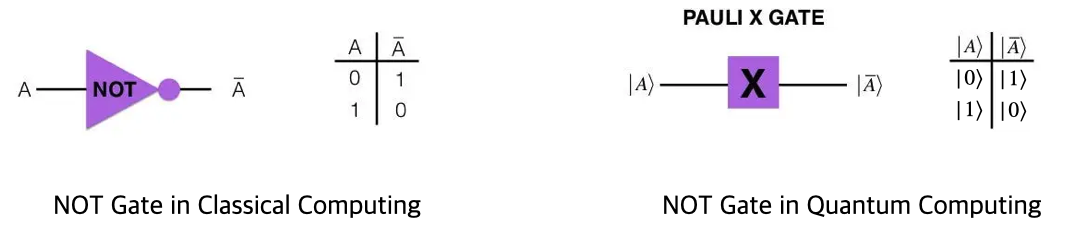
\includegraphics[width=0.8\linewidth]{figs/Not Gates.png}
    \caption{NOT Gates in Classical/Quantum Computing}
    \label{fig:NOT-Gates}
\end{figure}

고전 논리 회로에서 NOT 게이트는 [그림3.1]과 같이 input이 0인 경우 output으로 1을 내놓고, input이 1인 경우 output으로 0을 내놓는 역할을 한다. 이는 \(\mathbb{Z}_2\)에서 \( \text{NOT } A = A + 1\)과 같다.

양자 논리 회로에서 NOT Gate는 특별하게 Pauli-X Gate라고 불리며, [그림3.1]과 같이 input이 \(\ket 0\)인 경우 output으로 \(\ket 1\)을, input이 \(\ket 1\)인 경우 output으로 \(\ket 0\)을 내놓는 역할을 한다.

이 Operation은 다음과 같이 나타나는데:
\begin{align*}
    X\ket{0} &= \ket{1}  \\
    X\ket{1} &= \ket{0}
\end{align*}
따라서 \(X\)가 다음과 같은 matrix form을 가져야 함을 어렵지 않게 추론할 수 있다.
\[
    X = \begin{pmatrix}
        0 & 1 \\
        1 & 0
    \end{pmatrix}
\]
이와 같이, qubit state는 벡터이고, qubit에 가해지는 operation은 행렬로 나타난다.

\noindent 하지만 qubit state vector는 몇 가지 특별한 특징을 갖는다는 것을 알고 있다. 특히, qubit들은 normalize 되어야 한다. 즉, 길이가 1이다. 따라서 qubit에 작동하는 모든 matrix는 vector의 크기를 보존하는 구조를 필요로 한다. 선형대수학에서, 이러한 특징을 갖는 matrix를 Unitary Matrix라고 하며, Unitary Matrix는 다음과 같은 추가적인 필요충분조건을 갖는다.

\noindent \(\text{for } n \times n \text{ Unitary Matrix }U \text{, } {\sf TFAE} \)
\begin{flalign*}
    & \text{1. } U^\dagger = U^{-1} \\
    & \text{2. } UU^\dagger = U^\dagger U = I_n \\
    & \text{3. rows of } U \text{ are orthonormal} \\
    & \text{4. columns of } U \text{ are orthonormal} \\
    & \text{5. } {}^{\forall}\mathbf{x, y} \in \mathbb{C}^n, U\mathbf{x} \cdot U\mathbf{y} = \mathbf{x} \cdot \mathbf{y} \\
    & \text{6. } {}^{\forall}\mathbf{x} \in \mathbb{C}^n, || U\mathbf{x} || = || \mathbf{x} ||
\end{flalign*}
\noindent 가장 중요한 것은 1번째 성질로, \(U\)의 inverse \(U^{-1}\)는 \(U^\dagger\) 즉, \(U\)를 transpose하고, 모든 entry에 conjugate을 취한 것과 같다는 것이다.

\subsubsection{A.1.3.2 \quad Single Qubit Gates}
모든 qubit operation이 Unitary Matrix인 것과 같이, 모든 Unitary Matrix는 그 자체로 qubit operation이 된다. [표 3.1]과 같이 다양한 용도의 Unitary Operation이 존재한다:

\begin{table}[htb!]
    \centering
    \begin{tabular}{|c|c|c|c|c|}
        \hline
         Name & Symbol & Matrix & Basis state action \\ \hline

         Pauli-X & X & \(\begin{pmatrix} 0 & 1 \\ 1 & 0 \end{pmatrix}\) & \begin{tabular}[l]{@{}l@{}} $X\ket{0} = \ket{1}$\\ $X\ket{1} = \ket{0}$ \end{tabular} \\ \hline

         Pauli-Y & Y & \(\begin{pmatrix} 0 & -i \\ i & 0 \end{pmatrix}\) & \begin{tabular}[l]{@{}l@{}} $Y\ket{0} = i\ket{1}$\\ $Y\ket{1} = -i\ket{0}$ \end{tabular} \\ \hline

         Pauli-Z & Z & \(\begin{pmatrix} 1 & 0 \\ 0 & -1 \end{pmatrix}\) & \begin{tabular}[l]{@{}l@{}} $Z\ket{0} = \ket{0}$\\ $Z\ket{1} = -\ket{1}$ \end{tabular} \\ \hline

         Hadamard & H & \(\displaystyle {1\over\sqrt{2}}\begin{pmatrix} 1 & 1 \\ 1 & -1 \end{pmatrix}\) & \begin{tabular}[l]{@{}l@{}} $\displaystyle H\ket{0} = {1\over\sqrt{2}}\left(\ket{0} + \ket{1} \right) $ \\ $\displaystyle H\ket{1} = {1\over\sqrt{2}}\left(\ket{0} - \ket{1} \right) $ \end{tabular} \\ \hline

         S & S & \(\begin{pmatrix} 1 & 0 \\ 0 & i \end{pmatrix}\) & \begin{tabular}[l]{@{}l@{}} $S\ket{0} = \ket{0}$\\ $S\ket{1} = i\ket{1}$ \end{tabular} \\ \hline

         T & T & \(\begin{pmatrix} 1 & 0 \\ 0 & {e^{i\pi / 4}} \end{pmatrix}\) & \begin{tabular}[l]{@{}l@{}} $T\ket{0} = \ket{0}$\\ $T\ket{1} = e^{i\pi / 4}\ket{1}$ \end{tabular} \\ \hline

         $RX$ & $RX$ & \(\displaystyle \begin{pmatrix} \cos\left({\theta \over 2}\right) & -i\cdot\sin\left({\theta \over 2}\right) \\ -i\cdot\sin\left({\theta \over 2}\right) & \cos\left({\theta \over 2}\right) \end{pmatrix}\) & \begin{tabular}[l]{@{}l@{}} $\displaystyle RX(\theta) \ket{0} = \cos{\theta \over 2}\ket{0} -i\sin{\theta\over 2}\ket{1}$\\ $\displaystyle RX(\theta)\ket{1} = -i\sin{\theta \over 2}\ket{0} -\cos{\theta\over 2}\ket{1}$ \end{tabular} \\ \hline

         $RY$ & $RY$ & \(\displaystyle \begin{pmatrix} \cos\left({\theta \over 2}\right) & -\sin\left({\theta \over 2}\right) \\ \sin\left({\theta \over 2}\right) & \cos\left({\theta \over 2}\right) \end{pmatrix}\) & \begin{tabular}[l]{@{}l@{}} $\displaystyle RY(\theta) \ket{0} = \cos{\theta \over 2}\ket{0} + \sin{\theta\over 2}\ket{1}$\\ $\displaystyle RY(\theta)\ket{1} = -\sin{\theta \over 2}\ket{0} +\cos{\theta\over 2}\ket{1}$ \end{tabular} \\ \hline

         $RZ$ & $RZ$ & \(\displaystyle \begin{pmatrix} e^{-i{\theta \over 2}} & 0 \\ 0 & e^{i{\theta \over 2}} \end{pmatrix}\) & \begin{tabular}[l]{@{}l@{}} $\displaystyle RZ(\theta) \ket{0} = e^{-i{\theta \over 2}}\ket{0}$\\ $ RZ(\theta)\ket{1} = e^{i{\theta \over 2}}\ket{1}$ \end{tabular} \\ \hline
    \end{tabular}
    \caption{Single Qubit Gates : Matrix and Actions}
    \label{tab:single qubit gates}
\end{table}
[표 3.1]에 나타난 여러 Single Qubit Gate 중, Hadamard Gate는 \(\ket{0}\)에 적용했을 때 \(\ket 0\)과 \(\ket 1\)의 상태가 동일한 확률로 중첩되도록 하는 gate이다. 또한 RX, RY, RZ Gate의 동작을 이해하기 위해서는, 아래 식과 같이 single qubit state를 매개변수화하고, 이를 [그림 3.2]의 Bloch Sphere를 통해 시각화하면 그 동작이 직관적으로 이해된다:
% 또한 RX, RY, RZ Gate의 경우 다음과 같이 매개변수화된 single qubit state와, 이를 시각화한 Bloch Sphere를 통해 그 동작이 직관적으로 이해된다:
\[
    \ket{\psi(\theta, \phi)} = \cos{\left({\theta \over 2}\right)}\ket 0 + \sin{\left({\theta \over 2}\right)}e^{i\phi} \ket 1
\]
% \textit{global phase를 배제한 }
위와 같이 single qubit state를 변수 \(\theta, \phi\)에 대해 매개변수화하면, 구면좌표로 표현된 3차원 공간에서, qubit state와 unit vector간의 연관성을 만들 수 있다. 이 연관성을 통해 single qubit에서의 state 및 operation의 구조와 동작을 이해하는 시각화 도구인 Bloch Sphere([그림 3.2])가 고안되었다.
\begin{figure}[htb!]
    \centering
    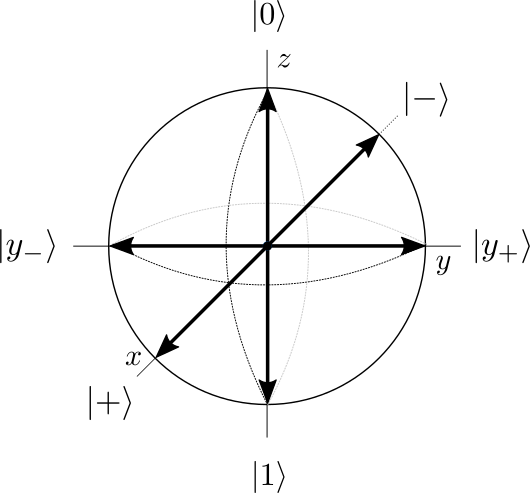
\includegraphics[width=0.5\linewidth]{figs/bloch_sphere.png}
    \caption{Bloch Sphere}
    \label{fig:bloch-sphere}
\end{figure}

\noindent Bloch Sphere에는 세 개의 축($x, y, z$)이 있다. z축에서, 맨 위의 상태는 $|0\rangle$, 맨 아래의 상태는 $|1\rangle$을 의미한다. 이는 Pauli Z operator의 eigenvector들이다. 유사하게, x축에는 $|+\rangle = {1\over \sqrt 2}\left(|0\rangle + |1\rangle\right)$, $|-\rangle = {1\over \sqrt 2}\left(|0\rangle - |1\rangle\right)$ 상태가 있고, 이는 Pauli X operator의 eigenvector들이다. y축에 대해서도 비슷한 결과를 얻을 수 있다.
\begin{figure}[htb!]
    \centering
    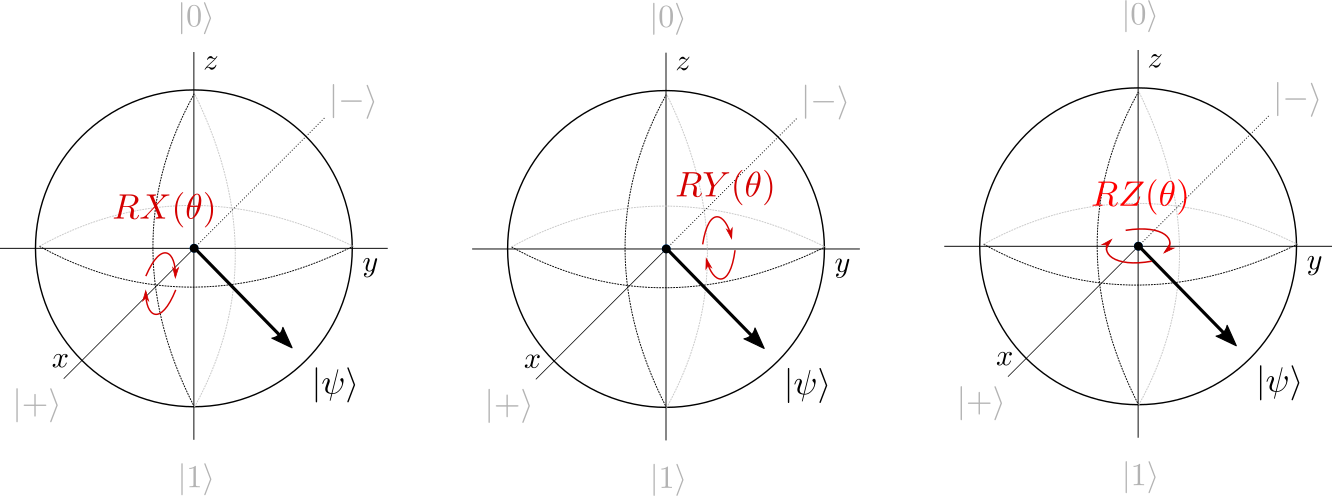
\includegraphics[width=1.0\linewidth]{figs/RXRYRZ.png}
    \caption{RX, RY, and RZ operations on Bloch Sphere}
    \label{fig:RX RY RZ}
\end{figure}

[그림 3.3]을 통해, RX, RY, RZ Gate의 동작에 대해 시각적으로 이해할 수 있다. Bloch Sphere 위의 한 점은 single qubit state 하나에 대응되고, RX, RY, RZ Gate는 주어진 매개변수 \(\theta\)만큼, 각 축에 대해 반시계방향으로 회전하는 것과 같다.

\subsubsection{A.1.3.3 \quad Universal Gate Set}
고전 논리 게이트에서, 모든 논리 게이트를 \(\{AND, OR, NOT\}\)의 조합으로 구성할 수 있으며 이를 Universal Gate Set이라고 한다. 양자 게이트도 마찬가지로 Universal Gate Set이 존재하는데, 모든 single qubit operation, 즉 모든 unitary를 구성하기 위해서는 [표 3.1] 중 \(\{RX, RY\}\), \(\{RY, RZ\}\), \(\{RZ, RX\}\)와 같이 \(\{RX, RY, RZ\}\) 중 2개의 operation을 선택하면, 그들의 조합만으로 모든 Unitary를 구성할 수 있다. 예컨대 \(\{RY, RZ\}\)만으로 모든 Unitary를 구성할 수 있음을 살펴보자.

\noindent 먼저, 모든 Unitary Matrix는 다음과 같이 3개의 매개변수 \(\phi, \theta, \omega\)로 표현이 가능하다.
\[
U(\phi, \theta, \omega) = \left( \begin{matrix}
 e^{-i(\phi + \omega)/2}\cos(\theta/2) & {-e^{i(\phi - \omega)/2}\sin(\theta/2) }
\\
 e^{-i(\phi - \omega)/2}\sin(\theta/2) & {e^{i(\phi + \omega)/2}\cos(\theta/2) }
\end{matrix}
\right)
\]

\noindent 이는 다음과 같이, \(RZ, RY\)으로 decompose될 수 있다.

\begin{align*}
    RZ(\omega)RY(\theta)RZ(\phi) &= \begin{pmatrix} e^{-i{\omega \over 2}} & 0 \\ 0 & e^{i{\omega \over 2}} \end{pmatrix} \begin{pmatrix} \cos\left({\theta \over 2}\right) & -\sin\left({\theta \over 2}\right) \\ \sin\left({\theta \over 2}\right) & \cos\left({\theta \over 2}\right) \end{pmatrix} \begin{pmatrix} e^{-i{\phi \over 2}} & 0 \\ 0 & e^{i{\phi \over 2}} \end{pmatrix} \\
    &= \begin{pmatrix} e^{-i{\omega \over 2}}\cos\left({\theta \over 2}\right) & -e^{-i{\omega \over 2}}\sin\left({\theta \over 2}\right) \\ e^{i{\omega \over 2}}\sin\left({\theta \over 2}\right) & e^{i{\omega \over 2}}\cos\left({\theta \over 2}\right) \end{pmatrix} \begin{pmatrix} e^{-i{\phi \over 2}} & 0 \\ 0 & e^{i{\phi \over 2}} \end{pmatrix} \\
    &= \begin{pmatrix}
     e^{-i(\phi + \omega)/2}\cos(\theta/2) & {-e^{i(\phi - \omega)/2}\sin(\theta/2) } \\
     e^{-i(\phi - \omega)/2}\sin(\theta/2) & {e^{i(\phi + \omega)/2}\cos(\theta/2) }
    \end{pmatrix} \\
    &= U(\phi, \theta, \omega) \quad \square
\end{align*}

이처럼 single qubit gate의 Universal Gate Set이 존재하고, 이는 양자 머신러닝의 General한 모델을 구성하는데 중요한 역할을 한다.

% --> Thm으로 쓰고 Proof를 넣을까? Proof 자체는 들어가긴 해야할 듯 Reference를 달던지

% 현재 시간 12월 3일 오전 2시 56분... 내일부턴 Universal Gate Set과(고민해보고) Multi-qubit gate 설명해야 함..

\subsubsection{A.1.3.4 \quad Multi Qubit Gate}
% 여러 qubit에 대한 연산은 두 가지 형태로 표현이 가능하다. 첫 번째 형태는 근본적으로 개별(individual) 큐비트에 대한 단일 큐비트 연산을 수행하는 것처럼 보이지만, 다중 큐비트 시스템에서는 여러 single qubit 연산을 병렬로 적용할 수 있다. 단순히 개별 큐비트 연산의 텐서 곱으로 표현될 수 있기 때문에 이를 분리 가능한 연산(seperable operation)이라고 부른다.

여러 qubit에 대한 연산은, qubit의 개수에 따라 그 크기에 맞는 Unitary Matrix로 이루어진다. 예컨대 2 qubit state의 경우 normalize된 4-dimension complex vector이고, 따라서 Quantum Gate로 \(4 \times 4\) Unitary Matrix를 사용한다. 이를 일반화하면, $n$ qubit state에 대한 Operation은 \(2^n \times 2^n\) Unitary Matrix를 사용함을 알 수 있다.

이러한 multi-qubit gate를 두 가지 종류로 분류할 수 있다. 첫 번째는 각각의 qubit에 독립적으로 single-qubit gate가 가해지는 것이고, 두 번째는 여러 qubit이 결부되어 operation이 가해지는 것이다.

\noindent 먼저 첫 번째 예시를 살펴보기 전에, 두 Matrix간의 tensor product를 정의한다.
\begin{definition}
Tensor product \(\otimes\) between Matrix

Let \( A \) and \( B \) be \(2 \times 2\) matrices defined as:
\[
A = \begin{pmatrix}
a_{11} & a_{12} \\
a_{21} & a_{22}
\end{pmatrix}, \quad
B = \begin{pmatrix}
b_{11} & b_{12} \\
b_{21} & b_{22}
\end{pmatrix}.
\]

The \textbf{tensor product} \( A \otimes B \) is defined as:
\[
A \otimes B =
\begin{pmatrix}
a_{11}B & a_{12}B \\
a_{21}B & a_{22}B
\end{pmatrix},
\]
where each entry \( a_{ij}B \) is a scalar multiple of the matrix \( B \).

Explicitly, we have:
\[
A \otimes B =
\begin{pmatrix}
a_{11}b_{11} & a_{11}b_{12} & a_{12}b_{11} & a_{12}b_{12} \\
a_{11}b_{21} & a_{11}b_{22} & a_{12}b_{21} & a_{12}b_{22} \\
a_{21}b_{11} & a_{21}b_{12} & a_{22}b_{11} & a_{22}b_{12} \\
a_{21}b_{21} & a_{21}b_{22} & a_{22}b_{21} & a_{22}b_{22}
\end{pmatrix}
\]

Likewise, for arbitrary matrices A(\(n_A \times m_A\)) and B(\(n_B \times m_B\)), tensor product \( A \otimes B \) is defined as:
\[
A \otimes B =
\begin{pmatrix}
a_{11}B & a_{12}B & \cdots & a_{1m_A}B \\
\vdots &          & \ddots & \vdots  \\
a_{n_A 1}B & a_{n_A 2}B & \cdots & a_{n_A m_A}B
\end{pmatrix}
\]
\end{definition}

\noindent 이제, 각 qubit에 독립적으로 가해지는 multi-qubit operation의 예시를 살펴보자.

\begin{example} % 당연하다는 듯이 써도 되나? 주의
multi-qubit gate as product of single-qubit gates

\noindent \(\ket{00} = \ket{0} \otimes \ket{0}\)과 같은 2 qubit state가 있다고 생각하자. 이때 첫 번째 qubit에 \(U_1\) gate, 두 번째 qubit에 \(U_2\) gate를 적용함을 생각하면, 다음과 같이 기술할 수 있다.

\[
\ket{00} \xrightarrow[]{U_1 \text{ for 1st qubit, } U_2 \text{ for 2nd qubit}} U_1\ket{0} \otimes U_2\ket{0}
\]

\noindent 이는 수학적으로 \((U_1 \otimes U_2)\ket{00}\)과 동일하며, 일반적인 multi-qubit gate에 대하여 성립한다.
\end{example}

다음으로, 여러 qubit이 결부된 multi-qubit gate의 예시로, CNOT(Controlled-NOT) gate를 살펴보자.
\begin{example}
CNOT gate as entangling gate

\[CNOT = \begin{pmatrix}
    1 & 0 & 0 & 0 \\
    0 & 1 & 0 & 0 \\
    0 & 0 & 0 & 1 \\
    0 & 0 & 1 & 0 \\
\end{pmatrix}\]

\noindent 위 행렬로 나타나는 CNOT gate는 다음 진리표([표 3.2])와 같이 작동하는데:

\begin{table}[htb!]
    \centering
    \begin{tabular}{|c|c|c|c|c|}
        \hline
         Input & Output \\ \hline
         $\ket{00}$ & $\ket{00}$ \\ \hline
         $\ket{01}$ & $\ket{01}$ \\ \hline
         $\ket{10}$ & $\ket{11}$ \\ \hline
         $\ket{11}$ & $\ket{10}$ \\ \hline
    \end{tabular}
    \caption{Operation of CNOT Gate}
    \label{tab:CNOT Operation}
\end{table}
진리표를 통해, 첫 번째 qubit(control bit라고 한다)의 state가 $\ket 1$이면 두 번째 qubit(target bit라고 한다)에 Pauli-X gate(NOT gate)를 동작시킨다는 것을 확인할 수 있다. 만약 control bit의 state가 $\ket 0$인 경우 아무런 동작도 하지 않는다.
\noindent $CNOT$ gate와 같이, 두 single-qubit unitary의 tensor product로 나타나지 않는 gate는 다양한 경우에 두 qubit 사이의 관계를 형성하게 되어 \textbf{entangling gate}라고 한다.
\end{example}

\noindent 또한 다음과 같이 일반적인 two-qubit Controlled-Unitary를 구성할 수 있다.

% \text{for } $U \in U(n)$,
\(\text{for } 2 \times 2 \text{ Unitary Matrix }U \text{,}\)

\[
    CU = \begin{pmatrix}
        I_2 & O \\
        O & U \\
    \end{pmatrix}
\]

위와 같이 정의된 two-qubit gate $CU$는, control bit인 첫 번째 qubit의 state가 $\ket 0$인 경우 아무런 동작도 하지 않고, control bit의 state가 $\ket 1$인 경우 target bit인 두 번째 qubit에 single-qubit gate $U$를 동작시킨다. 앞서 살펴본 $CNOT$ gate의 경우 위와 같이 일반적으로 정의된 $CU$에서 $U$에 Pauli-X를 대입한 것과 같다.

\noindent Quantum gate를 이해하기 위해, 마지막으로 다음 예시를 살펴보자.
\begin{example}
    Algorithm to make Bell State

먼저 two-qubit state \(\ket{00}\)를 준비하고, 다음 Step을 밟는다.
\begin{flalign*}
    & \text{1. 첫 번째 qubit에 Hadamard gate를 취한다.}  \\
    & \text{2. 첫 번째 qubit을 control bit, 두 번째 qubit을 target bit로 하는 CNOT gate를 취한다.}
\end{flalign*}
Step 1의 결과는 다음과 같다.
% \[
%     \ket{00} \xrightarrow[]{H \text{ for 1st qubit}} H\ket{0} \otimes \ket{0} = \left({\ket{0} + \ket{1} \over \sqrt{2}}\right) \otimes \ket{0}
% \]
\begin{flalign*}
    \ket{00} \xrightarrow[]{H \text{ for 1st qubit}} H\ket{0} \otimes \ket{0} &= \left({\ket{0} + \ket{1} \over \sqrt{2}}\right) \otimes \ket{0} \\
    &= {1\over \sqrt{2}}\left(\ket{00} + \ket{10}\right)
\end{flalign*}
즉, 첫 번째 qubit에는 $\ket 0$과 $\ket 1$이 동일한 확률로 중첩되어 있고, 두 번째 qubit은 원상태($\ket 0$)를 유지한다.

\noindent 다음으로, Step 2의 연산을 수행하면:
\[
    {CNOT}  \left({\ket{00} + \ket{10} \over \sqrt{2}} \right) = {\ket{00} + \ket{11} \over \sqrt{2}}
\]
즉, Step 1과 Step 2의 연산 결과 1번째 qubit의 state가 $\ket 0$이면 2번째 qubit의 state도 $\ket 0$이고, 1번째 qubit의 state가 $\ket 1$이면 2번째 qubit의 state도 $\ket 1$인 가장 기본적인 entangled state를 생성하게 된다. A.1.2절에서 살펴보았던, 이 state를 특별히 Bell State라고 한다.

\end{example}

\subsection{Quantum Circuit} % 마지막으로, 양자컴퓨팅의 개념 중 양자 회로에 대해 소개하고 이번 section을 마무리한다.
양자 회로(Quantum Circuit)는 양자 계산 중에 qubit에서 수행되는 일련의 작업들을 시각적으로 표현하는 일반적인 방법이다. 이들은 qubit(또는 wire라는 표현을 사용한다) 세트에 적용되는 연산 또는 게이트 세트로 구성된다. 양자 회로 다이어그램에서의 각 wire는 qubit을 나타낸다. 회로는 왼쪽에서 오른쪽으로 읽고, 이것은 operation이 적용되는 순서이다. 양자회로는 하나 이상의 큐비트의 측정(measurement)이 이루어지면 종료된다.

각 gate의 양자 회로 표현은 [그림 3.4]와 같다.
\begin{figure}[htb!]
    \centering
    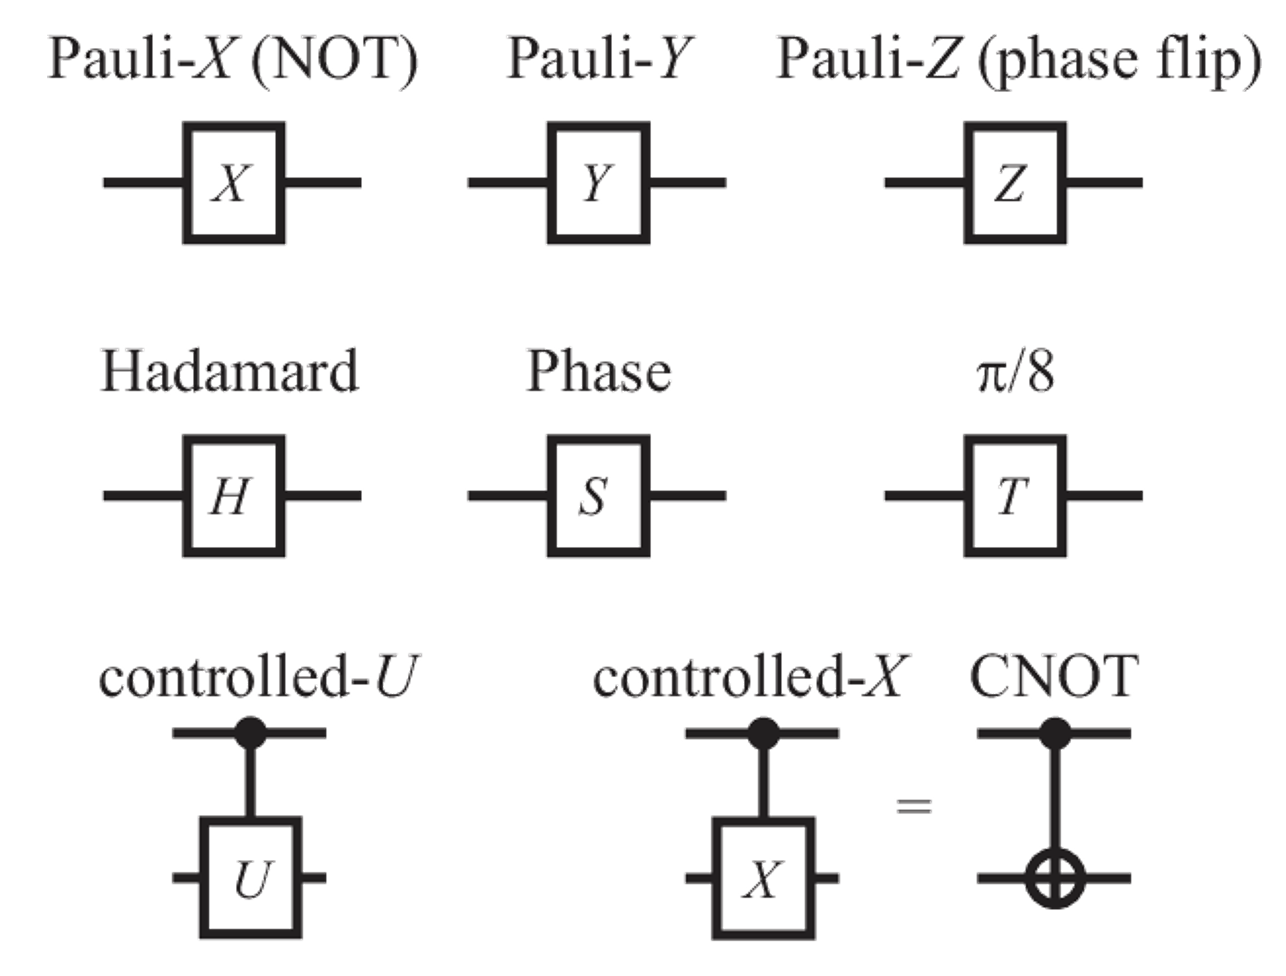
\includegraphics[width=0.45\linewidth]{figs/QuantumGateSymbols.png}
    \caption{Circuit representation of elementary quantum gates}
    \label{fig:quantum gate symbols}
\end{figure}

\begin{figure}[htb!]
    \centering
    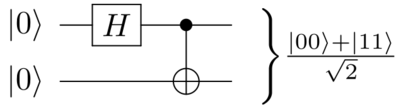
\includegraphics[width=0.5\linewidth]{figs/BellStateCircuit.png}
    \caption{Bell State Preparation Circuit}
    \label{fig:bell state circuit}
\end{figure}

[그림 3.5]는 Example 3.2.3에서의 연산과정을 양자회로로 표현한 것으로, 첫 번째 qubit에 Hadamard gate를, 이후 CNOT gate를 가동한 과정을 행렬식이나 bra-ket notation으로 표현한 것보다 직관적으로 이해할 수 있다.

양자 회로는 곧 양자 알고리즘이다. 보편적인 프로그래밍에서 알고리즘과 소프트웨어의 복잡도(complexity) 및 resource requirement를 고려하여 그 효율성을 높이는 것처럼, 양자 회로에 대해서도 동일한 과제가 주어진다. 양자 회로의 효율성을 평가하는 한 가지 중요한 기준은 바로 \textbf{Circuit Depth}이다. 여기서 Depth는, 가능한 한 병렬로 연산이 수행될 경우 회로가 작동하는 데 걸리는 시간 단계를 의미한다. 또는 회로의 layer 수라고 생각할 수 있다. 예컨대, [그림 3.5]에 나타난 회로의 경우 2의 depth를 가진다.

\subsection{Measurement and Expectation Value}
지금까지 quantum computer의 연산이 어떻게 동작되는지에 대해서 살펴보았다. 하지만 실제 문제를 해결하려고 하면, 일련의 알고리즘을 수행한 이후의 qubit state를 해석하여서 직면한 문제와 다시 연관시킬 수 있는 방법이 필요하다. 이에 전술한 것과 같이, 모든 양자 알고리즘은 다양한 방식으로의 병렬 연산을 수행한 후, 마지막으로 정보를 추출하기 위한 최종 단계를 거친다. 이때 마지막 정보 추출의 과정에 사용되는 연산은 Unitary 연산은 아니다. 따라서, 양자 알고리즘의 최종 단계인 Measurement와 Expectation Value에 대해 살펴보고 3.2장을 마친다.

\subsubsection{A.1.5.1 \quad Measurement}
다음과 같은 qubit state를 가정하자.
$$
|\psi \rangle = \alpha |0\rangle + \beta |1\rangle
$$
먼저, 이전에 살펴본 것은 위 qubit을 측정하면, $|0\rangle$으로 측정될 확률은 $|\alpha | ^2 = \alpha\alpha^*$이고, $|1\rangle$으로 측정될 확률은 $|\beta|^2$라는 것이다. measurement outcome probability를 표현하는 조금 더 formal한 방법은, inner product를 사용하는 것이다. quantum state $|\psi\rangle$가 주어지면, 그 state가 $|\phi \rangle$ state로 측정될 확률 \(\Pr(\phi)\)은 다음과 같다.% (basis that includes $|\phi \rangle$)
\begin{definition}
    probability that state \(\ket\psi\) is measured by state \(\ket\phi\)
$$
\Pr(\phi) = |\langle \phi |\psi \rangle | ^2
$$
\end{definition}
다음 예시를 살펴보자:
\begin{example}
    computing $\Pr(0)$ and $\Pr(1)$ for $|\psi\rangle = \alpha|0\rangle + \beta|1\rangle$
\[
\Pr(0) = |\langle0|\psi\rangle|^2 =|\langle0|(\alpha|0\rangle +\beta|1\rangle)|^2 = |\alpha \langle0|0\rangle + \beta \langle0|1\rangle|^2 = |\alpha|^2, \\
\]
\[
\Pr(1) = |\langle1|\psi\rangle|^2 =|\langle1|(\alpha|0\rangle +\beta|1\rangle)|^2 = |\alpha \langle1|0\rangle + \beta \langle1|1\rangle|^2 = |\beta|^2
\]
\end{example}
이때, 사용되는 measurement 방식을 특별히 projective measurement라고도 한다. 기본적으로, “각 basis state가 주어진 state에 얼마나 기여하는가?”를 묻고 있는 것이다. 이 이름은 두 state vector의 inner product 즉, 선형대수에서의 projection과 같은 연산을 수행하고 있다는 사실에서 기인한다. 그러나 standard linear algebra와 다른 한 가지 단계는, 실제 확률 값을 얻기 위해서는 inner product의 제곱을 취해야 한다는 것이다.

\subsubsection{A.1.5.2 \quad Expectation Value}

측정 결과로 확률 정보를 얻는 것은 qubit의 state에 따라 유용한 정보를 제공하지만, 종종은 그 state가 갖는 에너지와 같은 물리적인 것에 관심이 있을 때가 있다. 양자역학에는 에너지(energy), 운동량(momentum), 위치(position) 등 Observable이라는 이름의 "관측 가능한" 특성을 가지는 물리량이 존재한다. 이는 수학적으로, 임의의 양자 상태에 대해 Observable Operator의 기댓값(Expectation Value)이 실수값이라는 의미인데, 이는 다음과 같이 계산된다.
\begin{definition}
    Expectation Value of Observable \(A\) in the state \(\ket \psi\)
    \[
        \bra{\psi}A\ket{\psi}
    \]
\end{definition}

위 정의와 같이 주어진 Observable \(A\)에 대한 expectation value가 계산되는데, 이때 얻게 되는 값은 행렬 A의 eigenvalue와 각각의 확률에 대한 linear comination으로 나타난다. 따라서 Observable의 expectation value로 실수값만을 얻게 된다는 것은 Observable Matrix가 real eigenvalue만을 갖는다는 것이고, 이는 선형대수에서의 Hermitian matrix(\(A^\dagger = A\))에 해당한다.

\noindent 다음 예시를 살펴보자:

\begin{example} Calculating Expectation Value for given Observable

\[
    \text{For } |\psi\rangle = {4\over 5}|0\rangle - {3 \over 5}e^{i\pi / 3}|1\rangle,
\]
\[
\text{ suppose we want to measure the obsevable } B = \left( \begin{matrix}
    1 & -2i \\
    2i & 2
    \end{matrix}\right)
\]

\begin{align*}
    % & \text{i) eigenvalues of } B : \lambda_1 = 3.56155281 , \lambda_2 = -0.56155281 \\
    % & \text{ii) }
    \text{Expectation Value of } B : \langle\psi|B|\psi\rangle = {1 \over 25} \left(\begin{matrix}4 & -3e^{i\pi/3}\end{matrix}\right)\left(\begin{matrix}
        1 & -2i \\
        2i & 2
        \end{matrix}\right)\left(\begin{matrix} 4 \\ -3e^{i\pi /3}\end{matrix}\right) = -0.302769
\end{align*}

\end{example}
위 예시로 알아볼 수 있듯, 문제에 맞게 미리 구성한 Observable(Hermitian Matrix)를 이용하여, 보유한 quantum state에서 적절한 실수값을 추출할 수 있다. 이는 양자 머신러닝의 마지막 부분으로서 중요한 역할을 한다.


\section{Quantum Machine Learning} 

\subsection{Concepts}\label{qml:concepts}

앞으로 사용하게 될 주요한 용어와 정의에 대해서 설명할 것이다.

\subsubsection{Classical Machine learning} 1950년대, Arthur Samuel은 머신러닝을 "명시적으로 프로그래밍되지 않고 컴퓨터가 학습할 수 있는 능력을 부여하는 연구 분야"로 정의하였다\citep{schuld2015introduction}. 즉, 머신러닝은 입력과 출력에 대한 관계를 데이터를 통해 발견해내는 알고리즘이라고 볼 수 있다. 이러한 머신러닝 중 \textbf{nerual network} 와 \textbf{back propagation}를 통해 학습하는 방법을 \textbf{deep learning}이라고 부른다.

nerual network 중 대표적으로 언급되는 것은 \textbf{mutil layer perceptron} 이라는 모델이다. 이 모델은 연결된 뉴런 또는 노드의 시스템으로 구성된다.\cite{gardner1998artificial} 여기서 하나의 노드는 수학적 함수로 표현이 가능한 모델이다. 이 모델의 출력은 가중치 $\mathbf{w} \in \mathbb{R}^n $와의 입력벡터 $\mathbf{x} \in \mathbb{R}^n $ 내적과 편향 $b \in \mathbb{R}$의 덧셈이 활성화함수 혹은 비선형함수라고 불리는 함수에 통과하게 되어 형성된다.\cite{krenker2011introduction}
이를 표현한 그래프를 보면 쉽게 이해할 수 있다. % 모델, 모델 ... -> 모델의 출력 대신 노드의 출력?이 맞지 않을까 일단 보류

\begin{figure}[htb!]
   \centering
   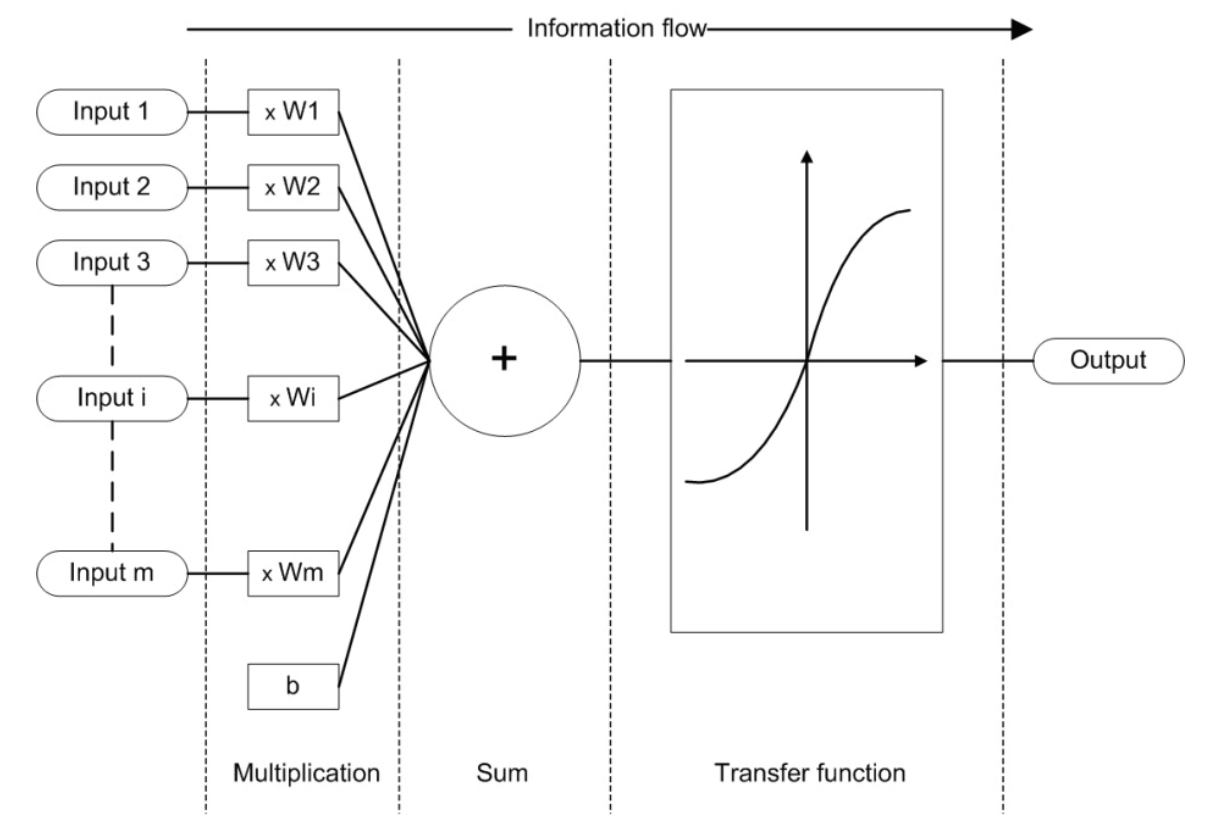
\includegraphics[width=0.8\textwidth]{figs/node.png}\
   \caption{Perceptron Architecture}
   \label{fig:node-image}
\end{figure}

이러한 노드들이 모이면 하나의 layer를 형성한다. 이렇게 형성된 layer 중 입력과 직접적으로 가중치 곱을 수행하는 layer를 \textbf{input layer}라고 하며, 최종적으로 노드의 출력이 마지막이 되는 layer를 \textbf{output layer}라고 한다. 그리고 input layer와 output layer 사이에 있는 layer들을 \textbf{hidden layer}라고 부른다.\cite{popescu2009multilayer} 이렇게 형성된 layer는 이전 layer의 노드들과 다음 layer의 노드들 간의 가중치 곱을 통해 연결되며, 이러한 가중치들은 이전 layer의 노드 개수 $N$, 다음 layer의 노드 개수 $M$ 과 함께 $N \times M $ 행렬로 표현된다. 이러한 가중치들은 bias와 함께 Backpropagation을 통해 학습 가능하기 때문에 \textbf{학습 파라미터}라고 불린다.

이렇게 형성된 multi perceptron layer는 다양한 비선형 함수를 근사할 수 있다는 장점과, 병렬연산이 가능한 행렬연산을 통한 빠른 추론, 입력데이터와 출력데이터를 범용적으로 선택할 수 있다는 장점 덕분에 많은 관심을 받았다.

\subsubsection{Components of Quantum Machine Learning}
quantum machine learning 분야는 지난 몇 년 동안 classical machine learning의 모델, 데이터 인코딩, 통계학적 방법등을 양자 알고리즘 및 양자정보이론을 통해 속도와 성능을 높이려는 노력과 함께 탄생하였다. 따라서 quantum machine learning은 입력 데이터와 출력 데이터의 관계를 찾아내어 가중치 혹은 파라미터를 학습시키는 양자 정보 처리 방법 중 하나라고 볼 수 있다.\cite{schuld2015introduction}. 여기서 나타나는 입력 데이터는 양자 정보 이론을 사용하기 위해 양자 컴퓨터가 처리 가능한 데이터로 변환하는 과정이 반드시 수행되어야 한다. 그러나 이를 수행하는 과정을 "input problem"이라고 할 만큼 계산량이 많기 때문에 중요한 과정이며 이를 개선하기 위한 연구들이 많이 진행되어왔다.\cite{biamonte2017quantum}

전술하였듯 양자컴퓨터가 처리가능한 데이터를 양자 데이터라고 부르는데, 이는 qubit들을 통해 처리 가능한 정보를 의미하며 양자상태, 양자 레지스터, 양자회로 등으로 다양하게 나타날 수 있다.이렇게 기존에 보유한 데이터를 양자 데이터로 전환하는 과정을 \textbf{qunatum encoding}이라고 하는데 encoding 방식에 따라 \textbf{angle encoding}, \textbf{basis encoding}, \textbf{amplitude encoding}으로 불리우며, quantum autoencoder와 같이 새로운 방식들이 등장하고 있다.\cite{rath2023quantum}

\textbf{basis encoding}은 이러한 encoding 방식 중 가장 간단한 방식이다. 이 방법은 고전 데이터를 그대로 qubit state의 텐서곱으로 표현하는 것이다. 예를 들어 고전 데이터 5(101)가 주어진다면, 이를 다음과 같은 방법으로 매핑된다고 볼 수 있다.
\[
5 \mapsto |101\rangle = |1\rangle \otimes |0\rangle \otimes |1\rangle
\]
이는 정수형이나 문자열 등 주로 이산적인 데이터를 다룰때 사용하는 방식이다.

\textbf{Angle Encoding}은 입력 데이터를 qubit state의 phase에 encoding하는 방식으로, qubit circuit을 통해 이를 효율적으로 다룰 수 있기 때문에 중요한 방법이다. 또한 이를 활용하여 파라미터를 circuit안에 넣어 학습시킬 수 있는 parameter quantum circuit에 사용되기 때문에 더욱 중요하다. angle encoding은 RX, RY, RZ와 같은 rotation gate를 통해 하나의 qubit에 하나의 angle $\theta$ 값을 encoding한다. 예컨대 single qubit gate에 RX gate를 통해 angle encoding된 state는 다음과 같이 나타난다. % PQC는 삭제 요망

\[
|\psi(\theta)\rangle = R_y(\theta)|0\rangle + e^{i\phi}R_y(\theta)|1\rangle
\]
여기서 $e^{i\phi}$는 phase factor라고 불리우는 amplitude이며, 여기에 있는 $\phi$는 경우에 따라 사용되거나 무시될수 있다. 이를 qubit이 $n$개, 입력데이터 $\theta$가 n개 주어졌을때를 일반화하면 다음과 같이 표현된다.
\[
       |\psi(\theta_1, \ldots, \theta_n)\rangle = \bigotimes_{i=1}^n (R_y(\theta_i)|0\rangle + e^{i\phi_i}R_y(\theta_i)|1\rangle)
\]

% \clearpage
\textbf{Amplitude Encoding}은 데이터를 quantum state의 amplitude에 Encoding하는 방법이다. 이러한 방법은 n개의 qubit으로 $N := 2^n$개의 basis state coefficients에 데이터를 최대 $N$개 encoding 한다. 이를 일반화하여 표현하면 다음과 같다\cite{maronese2022quantum}

\[
|\psi_x\rangle = \sum_{i=0}^{N-1} \frac{x_{i}}{\norm{x}} |i\rangle
\]
여기서 입력 데이터 $\mathbf{x}$는 보통 N차원의 벡터가 된다. 이러한 encoding 방식은 기하 급수적인 qubit 효율 덕분에, 많은 양의 데이터를 압축해서 사용할 수 있지만, complex amplitude들을 encoding 할 경우 n개의 qubit을 사용할때 $\mathcal{O}(2^n)$의 depth가 요구된다는 단점이 있다.\cite{mitsuda2024approximate}

\textbf{Parameterized Quantum Circuit(PQC)}는 이렇게 encoding된 quantum data를 문제에 맞는 output state로 변환하는 역할을 하는 양자 회로이다. PQC는 고전적인 머신러닝 모델과 유사한 방식으로 작동하며, 최적의 결과를 도출하기 위해 양자 회로의 매개변수가 조정된다.이를 n개의 qubit이 주어졌을 때를 일반화하면 다음과 같이 표현될 수 있다.
\[
|\psi\rangle = \prod_{\ell=1}^{m} W_{\ell} u_{\ell}(\theta_{\ell}) |\psi_0\rangle
\]
여기서 \( |\psi_0\rangle \)는 초기 양자 상태를 나타내며, \( m \)은 layer의 반복 횟수, \( W_{\ell} \)는 \(\ell\)-번째 레이어에서의 비매개변수화된 양자 게이트, \( U_{\ell}(\theta_{\ell}) \)는 매개변수 \(\{\theta_0, \theta_1, \ldots, \theta_k\}\)를 가지는 \(\ell\)-번째 레이어에서의 매개변수화된 양자 게이트를 나타낸다. 이러한 pqc 회로는 data encoding 과정을 제외하면, mlp와 동일한 구조이지만 더 적은 파라미터와의 연산을 통해 출력이 나오는 구조이기 때문에, mlp를 대체하여 성능을 높이려는 방식으로 연구가 진행되고 있다. 이러한 연구중 하나가 우리에게 동기를 주었던 QRF이며 해당 연구에서 실제로 mlp를 pqc를 전환하였을때, 속도와 성능의 개선되었다는 것을 실험으로 보였다.\cite{yang2022quantum}
% 이때, \( u_{\ell}(\theta_{\ell}) \)의 형태는 물리적 제약(예: 물리적 큐비트 간의 연결성 제한)에 따라 달라질 수 있다. 생략

%#########################################################
% 3.3.2 Components of QML
%
% Author : SEHYUN YUK
% Last Update: 2024.12.08
%
%##########################################################


%%%%%%%%%%%%%%%%%%%%%%%%%%%%%%%%% 2nd Lang Abstract %%%%%%%%%%%%%%%%%%%%%%%%%%%%%%%%%%%
% \setstretch{1.3} % ← of course you can change this as you wish, too.
% \chapter*{한국어 초록}\addcontentsline{toc}{chapter}{한국어 초록}%\setcounter{page}{3}
% {\small
% \quad 본문이 비한국어인 경우 반드시 한국어 초록 첨부. (해당연도의 도서관 규정 필독). 폰트사이즈 일관성을 위해 여기 예시의 한국어초록은 ``$\backslash$\texttt{small}'' 사용.

% ~\\
% \hangindent=2em
% \hangafter=2
% \textbf{주\,요\,어}: 소행성, 열적 모델링, 표토, 복사압, 편광---광학, 편광---적외선

% ~\\
% \noindent \textbf{학 \quad 번}: 2000-12345
% }

%%%%%%%%%%%%%%%%%%%%%%%%%%%%%%%%%%%%%%%%%%%%%%%%%%%%%%%%%%%%%%%%%%

%\chapter*{Acknowledgement}\\
%\twocolumn
\strangechapter{Ack}{Acknowledgement}\addcontentsline{toc}{chapter}{Acknowledgement}
\small
\footnotesize
\setstretch{1.1}
\setlength{\parskip}{0.3em}
Acknowledgement goes here. Hangul in Acknowledgement may use ``\texttt{$\backslash$kr}'': Hong Gildong (\kr{홍길동}).

ChatGPT says ``Both acknowledgment and acknowledgement are correct spellings. The only difference is that acknowledgment is the preferred American English spelling, while acknowledgement is the preferred British English spelling. You can use either one based on your preference or the style guide you're following.''



\end{document}